\chapter{Implementation strategies: evaluation and results}
\chaptermark{Implementation strategies: evaluation and results}
\label{chapter:exp_setup_results}
\minitoc

%%%%%%%%%%%%%%%%%%%%%%%%%%%%%%%%%%%%%%%%%%%%%%%%%%%%%%%%%%%%%%%%%%%%%%%%%%%%%%%%%%%%%%%%%%%%%%%
\section{Introduction}
The previous chapter presented two countermeasures against fault injection attacks and taking into account simple fault models, such as \textit{single-bit flip inside one register at a given clock cycle}. These countermeasures have been implemented by grouping the different DIFT-related registers in order to minimise the number of parity and redundancy bits. However, nowadays, studies~\cite{CGVCBLC-22-cardis,VDSPB-24-jce} have shown that is it possible to fault multiple bits precisely.

In this chapter, we present four different implementation's strategies of countermeasures to better protect the D-RI5CY mechanism against more complex fault models. Then, we evaluate each of these strategies in terms of security against more complex fault models. Finally, we compare them in terms of performance and area overhead. We implemented the minimisation of redundancy bits strategy in the last chapter. As shown in Chapter~\ref{chapter:countermeasures}, Hamming Code or even SECDED is better to use than just the simple parity for the correction and detection capacity. Hence, in this chapter, we do not implement others strategies for the simple parity protection. However, we present the results obtained from our simulations campaigns on the fault models considered in this chapter.

Section~\ref{section:chap6_faultmodels} introduces the different fault models considered.
Section~\ref{section:chap6_implem_strategies} introduces the four different strategies developed and assessed in this chapter. Some tables are in Appendix~\ref{app:strat_details} due to their size.
Section~\ref{section:chap6_evaluation} presents the security assessment of these four strategies by giving the results associated to each fault model and the use cases to each strategy, and evaluate them in terms of security, performance, and area overhead.
Finally, in Section~\ref{section:chap6_discussion}, we discuss the results obtained from these five strategies according to their performance and area overhead and give the limitations for each strategy.

%%%%%%%%%%%%%%%%%%%%%%%%%%%%%%%%%%%%%%%%%%%%%%%%%%%%%%%%%%%%%%%%%%%%%%%%%%%%%%%%%%%%%%%%%%%%%%%
\section{Fault models considered in this chapter}
\label{section:chap6_faultmodels}
In Chapter~\ref{chapter:countermeasures}, we presented the results of fault injection campaigns targeting \textit{a single bit-flip in one register at a given clock cycle}, and \textit{a single bit-flip in two registers at two distinct clock cycles}. We demonstrated that lightweight countermeasures, such as simple parity, Hamming Code, or SECDED version of Hamming Code, are effective in protecting our DIFT mechanism against single bit-flips occurring in one register at one clock cycle or in two registers at two distinct clock cycles.

In this chapter, we extend our analysis to consider an attacker capable of injecting faults into DIFT-related registers, leading to a \textit{single bit-flip in two registers at a given clock cycle}. Furthermore, we account for an attacker able to induce \textit{multi-bit faults in one register at a given clock cycle}, as well as, \textit{multi-bit faults in two registers at a given clock cycle}. These fault models, introduced in Chapter~\ref{chapter:fissa}, are exhaustively tested across registers ranging from 1-bit to 10-bit. Registers larger than 10 bits, such as the configuration registers TPR and TCR, are excluded due to their size. For instance, simulating an exhaustive attack on a single 32-bit register for one cycle would require $2^{32}$ simulations (i.e: \powerTwo{pow(32,2)}{0} simulations), and for the combination of two 32-bit registers, the number of simulations would reach $2^{32} \times 2^{32}$ which is too large to be simulated in a reasonnable time. However, it is worth noting that the biggest register after these two 32-bit registers is a 6-bit register (cf. Table~\ref{tab:strategies_register_info}), so we fault every 1-bit to 6-bit registers.

The three fault models are exhaustively simulated across all possible values of these registers. To meet this objective, any DIFT-related register that maintains a 1-bit tag value, drives tag propagation or tag update processes, or holds security policy configurations, can be targeted. Additionally, registers storing redundancy bits for protection mechanisms are also considered.

% %%%%%%%%%%%%%%%%%%%%%%%%%%%%%%%%%%%%%%%%%%%%%%%%%%%%%%%%%%%%%%%%%%%%%%%%%%%%%%%%%%%%%%%%%%%%%%%
\section{Implementation strategies}
\label{section:chap6_implem_strategies}

Assessing the robustness of DIFT against more complex fault models requires comprehensive strategies that can identify vulnerabilities to enhance the system integrity. This section introduces four distinct strategies aimed at evaluating and enhancing the security of DIFT mechanisms against complex fault models. Each strategy offers a unique perspective on detecting, mitigating, or preventing the effects of multi bit-flip faults, contributing to a holistic approach in fortifying DIFT systems. By exploring these methodologies, we aim to provide actionable insights for developing more resilient DIFT solutions thanks to lightweight countermeasures.

\subsection{Strategy 2: Pipeline Stage Register Coupling for Robust Error Mitigation}

\begin{table}[t]
    \centering
    \scriptsize
    \caption{D-RI5CY Registers Details List for Strategy 2}
    \label{tab:strategy_2_register_info}
    % \setlength{\tabcolsep}{5pt}
    \begin{tabular}{@{}rccc@{}}
        \toprule
        Register Name                   & Module                                & Size   & \tableTwoLines{Strategy}{2} \\\midrule
        pc\_id\_o\_tag                  & \textcolor{red}{Instruction}          & 1      & Gr1                         \\
        pc\_if\_o\_tag                  & \textcolor{red}{Fetch Stage}          & 1      & Gr1                         \\\hdashline
        alu\_operand\_a\_ex\_o\_tag     &                                       & 1      & Gr2                         \\
        alu\_operand\_b\_ex\_o\_tag     &                                       & 1      & Gr2                         \\
        alu\_operand\_c\_ex\_o\_tag     &                                       & 1      & Gr2                         \\
        alu\_operator\_o\_mode          &                                       & 2      & Gr2                         \\
        check\_d\_o\_tag                &                                       & 1      & Gr2                         \\
        check\_s1\_o\_tag               &                                       & 1      & Gr2                         \\
        check\_s2\_o\_tag               & \textcolor{blue}{Instruction}         & 1      & Gr2                         \\
        is\_store\_post\_o\_tag         & \textcolor{blue}{Decode Stage}        & 1      & Gr2                         \\
        memory\_set\_o\_tag             &                                       & 1      & Gr2                         \\
        regfile\_alu\_waddr\_ex\_o\_tag &                                       & 5      & Gr2                         \\
        register\_set\_o\_tag           &                                       & 1      & Gr2                         \\
        store\_dest\_addr\_ex\_o\_tag   &                                       & 1      & Gr2                         \\
        store\_source\_ex\_o\_tag       &                                       & 1      & Gr2                         \\
        use\_store\_ops\_ex\_o          &                                       & 1      & Gr2                         \\\hdashline
        rf\_reg[0]                      &                                       & 1      & Gr3                         \\
        rf\_reg[1]                      &                                       & 1      & Gr3                         \\
        rf\_reg[2]                      & \textcolor{LimeGreen}{Register File}  & 1      & Gr3                         \\
        \ldots                          & \textcolor{LimeGreen}{Tag}            & \ldots & Gr3                         \\
        rf\_reg[30]                     &                                       & 1      & Gr3                         \\
        rf\_reg[31]                     &                                       & 1      & Gr3                         \\\hdashline
        rs1\_o\_tag                     & \textcolor{DarkOrange}{Execute Stage} & 1      & Gr4                         \\\hdashline
        tcr\_q                          & \textcolor{DarkRed}{Control and}      & 32     & Gr5                         \\
        tpr\_q                          & \textcolor{DarkRed}{Status Registers} & 32     & Gr6                         \\\hdashline
        data\_type\_q\_tag              &                                       & 2      & Gr7                         \\
        data\_we\_q\_tag                & \textcolor{magenta}{Load/Store}       & 1      & Gr7                         \\
        rdata\_offset\_q\_tag           & \textcolor{magenta}{Unit}             & 2      & Gr7                         \\
        rdata\_q\_tag                   &                                       & 4      & Gr7                         \\
        \bottomrule
    \end{tabular}
\end{table}

In the second implemented strategy, we rely on protecting each pipeline stage of our processor individually. To achieve this implementation, we decided to form seven groups: Instruction Fetch (IF) Stage, Instruction Decode (ID) Stage, Register File Tag, Execute (EX) Stage, two groups for the two registers TPR and TCR containing the security policy, and a last group with the Load/Store Unit. 

Table~\ref{tab:strategy_2_register_info} represents the different DIFT-related registers with their associated group.
Table~\ref{tab:strategy_2_groups} represents the number of protected bits inside each pipeline stage and their associated number of redundancy and parity bits, in the case of when SECDED is used. As depicted in this table, the number of protected bits differs a lot depending on the pipeline stage, ranging from one bit to thirty-two bits.
Otherwise, the HDL implementations are the same than Chapter~\ref{chapter:countermeasures} with two proposed implementations (see Figure~\ref{fig:implementation_sd_1} and Figure~\ref{fig:implementation_sd_2}). This strategy protects 107 bits by adding 30 redundancy bits and 7 parity bits which led to approximatively a 30\% increase in number of bits stored into registers.

\subsection{Strategy 3: Individual Register Encapsulation for Robust Error Mitigation}

\begin{table}[t]
    \centering
    \scriptsize
    \caption{D-RI5CY Registers Details List for Strategy 3}
    \label{tab:strategy_3_register_info}
    % \setlength{\tabcolsep}{5pt}
    \begin{tabular}{@{}rccc@{}}
        \toprule
        Register Name                   & Module                                & Size   & \tableTwoLines{Strategy}{3} \\\midrule
        pc\_if\_o\_tag                  & \textcolor{red}{Fetch Stage}          & 1      & Gr1                         \\
        pc\_id\_o\_tag                  & \textcolor{red}{Instruction}          & 1      & Gr2                         \\\hdashline
        alu\_operand\_a\_ex\_o\_tag     &                                       & 1      & Gr3                         \\
        alu\_operand\_b\_ex\_o\_tag     &                                       & 1      & Gr4                         \\
        alu\_operand\_c\_ex\_o\_tag     &                                       & 1      & Gr5                         \\
        alu\_operator\_o\_mode          &                                       & 2      & Gr6                         \\
        check\_d\_o\_tag                &                                       & 1      & Gr7                         \\
        check\_s1\_o\_tag               &                                       & 1      & Gr8                         \\
        check\_s2\_o\_tag               & \textcolor{blue}{Instruction}         & 1      & Gr9                         \\
        is\_store\_post\_o\_tag         & \textcolor{blue}{Decode Stage}        & 1      & Gr10                        \\
        memory\_set\_o\_tag             &                                       & 1      & Gr11                        \\
        regfile\_alu\_waddr\_ex\_o\_tag &                                       & 5      & Gr12                        \\
        register\_set\_o\_tag           &                                       & 1      & Gr13                        \\
        store\_dest\_addr\_ex\_o\_tag   &                                       & 1      & Gr14                        \\
        store\_source\_ex\_o\_tag       &                                       & 1      & Gr15                        \\
        use\_store\_ops\_ex\_o          &                                       & 1      & Gr16                        \\\hdashline
        rf\_reg[0]                      &                                       & 1      & Gr17                        \\
        rf\_reg[1]                      &                                       & 1      & Gr17                        \\
        rf\_reg[2]                      & \textcolor{LimeGreen}{Register File}  & 1      & Gr17                        \\
        \ldots                          & \textcolor{LimeGreen}{Tag}            & \ldots & Gr17                        \\
        rf\_reg[30]                     &                                       & 1      & Gr17                        \\
        rf\_reg[31]                     &                                       & 1      & Gr17                        \\\hdashline
        rs1\_o\_tag                     & \textcolor{DarkOrange}{Execute Stage} & 1      & Gr18                        \\\hdashline
        tcr\_q                          & \textcolor{DarkRed}{Control and}      & 32     & Gr19                        \\
        tpr\_q                          & \textcolor{DarkRed}{Status Registers} & 32     & Gr20                        \\\hdashline
        data\_type\_q\_tag              &                                       & 2      & Gr21                        \\
        data\_we\_q\_tag                & \textcolor{magenta}{Load/Store}       & 1      & Gr22                        \\
        rdata\_offset\_q\_tag           & \textcolor{magenta}{Unit}             & 2      & Gr23                        \\
        rdata\_q\_tag                   &                                       & 4      & Gr24                        \\
        \bottomrule
    \end{tabular}
\end{table}

In the third implementation strategy, we aim to enhance protection for every register associated to the DIFT within our processor. To achieve this, we created 24 groups for all the registers, ensuring a more targeted and effective protection mechanism. The grouping was done based on each of them. Specifically, two groups were formed in the IF stage, addressing the initial handling of PC addresses. A significant portion, fourteen groups, was allocated to the ID stage, as this stage contains processing and handling of tags information. Additionally, one group was dedicated to the Register File Tag, as we consider this Register File as one register even if it is 32 registers to avoid an increase overhead for the Register File. For the EX stage, we formed a single group. Furthermore, two separated groups were created for the TPR and TCR registers, recognising their distinct control functions. Finally, four groups were designated for the Load/Store Unit, as it can be considered as the fourth stage of our processor. This structure allows for a granular protection approach, ensuring that each aspect of the processor's DIFT-related registers is securely managed. The issue with this strategy is the use of two redundancy bits and one parity bit to protect only one register bit.

Table~\ref{tab:strategy_3_register_info} represents the group composition with the different DIFT-related registers.
Table~\ref{tab:strategy_3_groups} represents the number of protected bits inside each protected group and their associated number of redundancy and parity bits, when SECDED is used. As depicted in this table, there is mainly only one bit protected in the majority of groups (16 groups over 24). This strategy protects 107 bits by adding 64 redundancy bits and 24 parity bits which led to approximatively a 70\% increase in number of bits stored into registers.

\subsection{Strategy 4: DIFT-Enhanced CSR Register Spliting for Strengthened Security}

\begin{table}[t]
    \centering
    \scriptsize
    \caption{D-RI5CY Registers Details List for Strategy 4}
    \label{tab:strategy_4_register_info}
    % \setlength{\tabcolsep}{5pt}
    \begin{tabular}{@{}rccc@{}}
        \toprule
        Register Name                   & Module                                & Size   & \tableTwoLines{Strategy}{3} \\\midrule
        pc\_if\_o\_tag                  & \textcolor{red}{Fetch Stage}          & 1      & Gr1                         \\
        pc\_id\_o\_tag                  & \textcolor{red}{Instruction}          & 1      & Gr2                         \\\hdashline
        alu\_operand\_a\_ex\_o\_tag     &                                       & 1      & Gr3                         \\
        alu\_operand\_b\_ex\_o\_tag     &                                       & 1      & Gr4                         \\
        alu\_operand\_c\_ex\_o\_tag     &                                       & 1      & Gr5                         \\
        alu\_operator\_o\_mode          &                                       & 2      & Gr6                         \\
        check\_d\_o\_tag                &                                       & 1      & Gr7                         \\
        check\_s1\_o\_tag               &                                       & 1      & Gr8                         \\
        check\_s2\_o\_tag               & \textcolor{blue}{Instruction}         & 1      & Gr9                         \\
        is\_store\_post\_o\_tag         & \textcolor{blue}{Decode Stage}        & 1      & Gr10                        \\
        memory\_set\_o\_tag             &                                       & 1      & Gr11                        \\
        regfile\_alu\_waddr\_ex\_o\_tag &                                       & 5      & Gr12                        \\
        register\_set\_o\_tag           &                                       & 1      & Gr13                        \\
        store\_dest\_addr\_ex\_o\_tag   &                                       & 1      & Gr14                        \\
        store\_source\_ex\_o\_tag       &                                       & 1      & Gr15                        \\
        use\_store\_ops\_ex\_o          &                                       & 1      & Gr16                        \\\hdashline
        rf\_reg[0]                      &                                       & 1      & Gr17                        \\
        rf\_reg[1]                      &                                       & 1      & Gr17                        \\
        rf\_reg[2]                      & \textcolor{LimeGreen}{Register File}  & 1      & Gr17                        \\
        \ldots                          & \textcolor{LimeGreen}{Tag}            & \ldots & Gr17                        \\
        rf\_reg[30]                     &                                       & 1      & Gr17                        \\
        rf\_reg[31]                     &                                       & 1      & Gr17                        \\\hdashline
        rs1\_o\_tag                     & \textcolor{DarkOrange}{Execute Stage} & 1      & Gr18                        \\\hdashline
        tpr\_q                          & \textcolor{DarkRed}{Control and}      & 32     & Gr19 - Gr26                 \\
        tcr\_q                          & \textcolor{DarkRed}{Status Registers} & 32     & Gr27 - Gr34                 \\\hdashline
        data\_type\_q\_tag              &                                       & 2      & Gr35                        \\
        data\_we\_q\_tag                & \textcolor{magenta}{Load/Store}       & 1      & Gr36                        \\
        rdata\_offset\_q\_tag           & \textcolor{magenta}{Unit}             & 2      & Gr37                        \\
        rdata\_q\_tag                   &                                       & 4      & Gr38                        \\
        \bottomrule
    \end{tabular}
\end{table}

In the fourth implementation, we stay with the protection on each register individually. However, we improve the protection on the two CSRs registers. Our idea is to split these two registers by group of operations (arithmetic, branching, etc. -- see Table~\ref{tab:tpr} and table~\ref{tab:tcr} for more details). In this way, we aim to enhance the detection of errors occurring in the security policy related registers.

Table~\ref{tab:strategy_4_register_info} shows the group affectation for each register. As TPR and TCR are split, they take eight groups each.
Table~\ref{tab:strategy_4_groups} depicts the number of redundancy and parity bits for each group. As the different operations of TPR and TCR are on one to four bits the number of redundancy bits vary from two to three. This strategy protects 103 bits by adding 101 redundancy bits and 38 parity bits which led to approximatively a 109\% increase in number of bits stored into registers.

\subsection{Strategy 5: Sliced Register Bit Coupling for Improved Data Integrity}

\begin{figure}[ht]
    \centering
    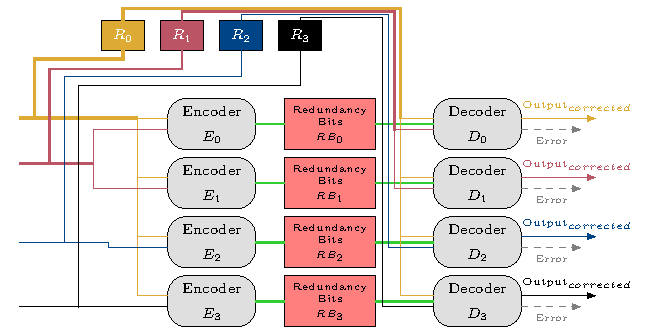
\includegraphics[page=1]{c6_group_composition/img/implem5_spaghetti.pdf}
    \caption{Strategy 5 -- Mixing Registers Implementation}
    \label{fig:strategy_5_functionning}
\end{figure}

\begin{table}[t]
    \centering
    \scriptsize
    \caption{D-RI5CY Registers Details List for Strategy 5}
    \label{tab:strategy_5_register_info}
    \begin{tabular}{@{}rccc@{}}
        \toprule
        Register Name                   & Module                                & Size   & \tableTwoLines{Strategy}{3} \\\midrule
        pc\_if\_o\_tag                  & \textcolor{red}{Fetch Stage}          & 1      & Gr1                         \\
        pc\_id\_o\_tag                  & \textcolor{red}{Instruction}          & 1      & Gr1                         \\\hdashline
        alu\_operand\_a\_ex\_o\_tag     &                                       & 1      & Gr4                         \\
        alu\_operand\_b\_ex\_o\_tag     &                                       & 1      & Gr5                         \\
        alu\_operand\_c\_ex\_o\_tag     &                                       & 1      & Gr6                         \\
        alu\_operator\_o\_mode          &                                       & 2      & Gr2 - Gr3                   \\
        check\_d\_o\_tag                &                                       & 1      & Gr9                         \\
        check\_s1\_o\_tag               &                                       & 1      & Gr7                         \\
        check\_s2\_o\_tag               & \textcolor{blue}{Instruction}         & 1      & Gr8                         \\
        is\_store\_post\_o\_tag         & \textcolor{blue}{Decode Stage}        & 1      & Gr10                        \\
        memory\_set\_o\_tag             &                                       & 1      & Gr11                        \\
        regfile\_alu\_waddr\_ex\_o\_tag &                                       & 5      & Gr5 - Gr9                   \\
        register\_set\_o\_tag           &                                       & 1      & Gr10                        \\
        store\_dest\_addr\_ex\_o\_tag   &                                       & 1      & Gr2                         \\
        store\_source\_ex\_o\_tag       &                                       & 1      & Gr3                         \\
        use\_store\_ops\_ex\_o          &                                       & 1      & Gr4                         \\\hdashline
        rf\_reg[0]                      &                                       & 1      & Gr12                        \\
        rf\_reg[1]                      &                                       & 1      & Gr12                        \\
        rf\_reg[2]                      & \textcolor{LimeGreen}{Register File}  & 1      & Gr12                        \\
        \ldots                          & \textcolor{LimeGreen}{Tag}            & \ldots & Gr12                        \\
        rf\_reg[30]                     &                                       & 1      & Gr12                        \\
        rf\_reg[31]                     &                                       & 1      & Gr12                        \\\hdashline
        rs1\_o\_tag                     & \textcolor{DarkOrange}{Execute Stage} & 1      & Gr35                        \\\hdashline
        tpr\_q                          & \textcolor{DarkRed}{Control and}      & 32     & Gr13 - Gr26 / Gr28 - Gr30   \\
        tcr\_q                          & \textcolor{DarkRed}{Status Registers} & 32     & Gr13 - Gr34                 \\\hdashline
        data\_type\_q\_tag              &                                       & 2      & Gr36 - Gr37                 \\
        data\_we\_q\_tag                & \textcolor{magenta}{Load/Store}       & 1      & Gr39                        \\
        rdata\_offset\_q\_tag           & \textcolor{magenta}{Unit}             & 2      & Gr37 - Gr38                 \\
        rdata\_q\_tag                   &                                       & 4      & Gr35 - Gr36 / Gr38 - Gr39   \\
        \bottomrule
    \end{tabular}
\end{table}

In the fifth strategy, we propose a less straightforward idea. Instead of protecting registers individually or by pipeline stage, we could protect them by mixing them. By mixing the registers, an attacker would require to attack precisely one bit of two different registers or more. Figure~\ref{fig:strategy_5_functionning} presents this strategy with four registers: one 4-bit register (i.e $R_0$), one 2-bit register (i.e $R_1$) and two 1-bit registers (i.e $R_2$ and $R_3$). Then we take the larger register and we decompose each bit into one Hamming Code or SECDED encoder and we add one bit of another register to this encoder. Each of these encoder take maximum as inputs two bits. If possible, we try to never mix the same registers together. In the following, the encoder and decoder computes in the same manner than other strategies. This strategy is longer to implement as it requires to separate each registers into different encoders. In our strategy, we have 39 encoders.

Table~\ref{tab:strategy_5_register_info} shows the group affectation for each register. For example, register \texttt{pc\_if\_o\_tag} is in group 1 only because it is a 1-bit register, while \texttt{regfile\_alu\_waddr\_ex\_o\_tag} is present in group 5 to group 9 because it is a 5-bit register. For the TPR we encode only the used bits: 0 to 13 and 15 to 17.
Table~\ref{tab:strategy_5_groups} presents the number of redundancy and parity bits for each group. This strategy protects 102 bits by adding 114 redundancy bits and 39 parity bits which led to a 120\% increase in number of bits stored into registers.

%%%%%%%%%%%%%%%%%%%%%%%%%%%%%%%%%%%%%%%%%%%%%%%%%%%%%%%%%%%%%%%%%%%%%%%%%%%%%%%%%%%%%%%%%%%%%%%
\section{Experimental results}
\label{section:chap6_evaluation}

\begin{table}[t]
    \centering
    \scriptsize
    \caption{D-RI5CY Registers Details List}
    \label{tab:strategies_register_info}
    \setlength{\tabcolsep}{4pt}
    \begin{tabular}{@{}rccccccc@{}}
        \toprule
        Register Name                   & Module                                & Size   & \tableTwoLines{Strategy}{1} & \tableTwoLines{Strategy}{2} & \tableTwoLines{Strategy}{3} & \tableTwoLines{Strategy}{4} & \tableTwoLines{Strategy}{5}                \\
        \midrule
        pc\_id\_o\_tag                  & \textcolor{red}{Instruction}          & 1      & Gr5                         & Gr1                         & Gr1                         & Gr1                         & Gr1                                        \\
        pc\_if\_o\_tag                  & \textcolor{red}{Fetch Stage}          & 1      & Gr5                         & Gr1                         & Gr2                         & Gr2                         & Gr1                                        \\\hdashline
        alu\_operand\_a\_ex\_o\_tag     &                                       & 1      & Gr5                         & Gr2                         & Gr3                         & Gr3                         & Gr4                                        \\
        alu\_operand\_b\_ex\_o\_tag     &                                       & 1      & Gr5                         & Gr2                         & Gr4                         & Gr4                         & Gr5                                        \\
        alu\_operand\_c\_ex\_o\_tag     &                                       & 1      & Gr5                         & Gr2                         & Gr5                         & Gr5                         & Gr6                                        \\
        alu\_operator\_o\_mode          &                                       & 2      & Gr5                         & Gr2                         & Gr6                         & Gr6                         & Gr2 - Gr3                                  \\
        check\_d\_o\_tag                &                                       & 1      & Gr5                         & Gr2                         & Gr7                         & Gr7                         & Gr9                                        \\
        check\_s1\_o\_tag               &                                       & 1      & Gr5                         & Gr2                         & Gr8                         & Gr8                         & Gr7                                        \\
        check\_s2\_o\_tag               & \textcolor{blue}{Instruction}         & 1      & Gr5                         & Gr2                         & Gr9                         & Gr9                         & Gr8                                        \\
        is\_store\_post\_o\_tag         & \textcolor{blue}{Decode Stage}        & 1      & Gr5                         & Gr2                         & Gr10                        & Gr10                        & Gr10                                       \\
        memory\_set\_o\_tag             &                                       & 1      & Gr5                         & Gr2                         & Gr11                        & Gr11                        & Gr11                                       \\
        regfile\_alu\_waddr\_ex\_o\_tag &                                       & 5      & Gr4                         & Gr2                         & Gr12                        & Gr12                        & Gr5 - Gr9                                  \\
        register\_set\_o\_tag           &                                       & 1      & Gr5                         & Gr2                         & Gr13                        & Gr13                        & Gr10                                       \\
        store\_dest\_addr\_ex\_o\_tag   &                                       & 1      & Gr5                         & Gr2                         & Gr14                        & Gr14                        & Gr2                                        \\
        store\_source\_ex\_o\_tag       &                                       & 1      & Gr5                         & Gr2                         & Gr15                        & Gr15                        & Gr3                                        \\
        use\_store\_ops\_ex\_o          &                                       & 1      & Gr5                         & Gr2                         & Gr16                        & Gr16                        & Gr4                                        \\\hdashline
        rf\_reg[0]                      &                                       & 1      & Gr3                         & Gr3                         & Gr17                        & Gr17                        & Gr12                                       \\
        rf\_reg[1]                      &                                       & 1      & Gr3                         & Gr3                         & Gr17                        & Gr17                        & Gr12                                       \\
        rf\_reg[2]                      & \textcolor{LimeGreen}{Register File}  & 1      & Gr3                         & Gr3                         & Gr17                        & Gr17                        & Gr12                                       \\
        \ldots                          & \textcolor{LimeGreen}{Tag}            & \ldots & Gr3                         & Gr3                         & Gr17                        & Gr17                        & Gr12                                       \\
        rf\_reg[30]                     &                                       & 1      & Gr3                         & Gr3                         & Gr17                        & Gr17                        & Gr12                                       \\
        rf\_reg[31]                     &                                       & 1      & Gr3                         & Gr3                         & Gr17                        & Gr17                        & Gr12                                       \\\hdashline
        rs1\_o\_tag                     & \textcolor{DarkOrange}{Execute Stage} & 1      & Gr5                         & Gr4                         & Gr18                        & Gr18                        & Gr35                                       \\\hdashline
        tcr\_q                          & \textcolor{DarkRed}{Control and}      & 32     & Gr1                         & Gr5                         & Gr19                        & Gr19 - Gr26                 & \tableTwoLines{Gr13 - Gr26 /}{Gr28 - Gr30} \\
        tpr\_q                          & \textcolor{DarkRed}{Status Registers} & 32     & Gr2                         & Gr6                         & Gr20                        & Gr27 - Gr34                 & Gr13 - Gr34                                \\\hdashline
        data\_type\_q\_tag              &                                       & 2      & Gr5                         & Gr7                         & Gr21                        & Gr35                        & Gr36 - Gr37                                \\
        data\_we\_q\_tag                & \textcolor{magenta}{Load/Store}       & 1      & Gr5                         & Gr7                         & Gr22                        & Gr36                        & Gr39                                       \\
        rdata\_offset\_q\_tag           & \textcolor{magenta}{Unit}             & 2      & Gr5                         & Gr7                         & Gr23                        & Gr37                        & Gr37 - Gr38                                \\
        rdata\_q\_tag                   &                                       & 4      & Gr5                         & Gr7                         & Gr24                        & Gr38                        & \tableTwoLines{Gr35 - Gr36 /}{Gr38 - Gr39} \\
        \bottomrule
    \end{tabular}
\end{table}

\begin{table}[t]
    \centering
    \footnotesize
    \caption{Registers by Strategy (SECDED count): Summary of Number and Size}
    \label{tab:strategies_summary}
    \begin{tabular}{rcc}
        \toprule
        Strategy            & Number of Registers & Number of Bits                                            \\
        \midrule
        Baseline -- D-RI5CY & 55                  & 127 {\scriptsize {\tiny (0\%)}                                 } \\
        Strategy 1          & 65                  & 157 {\scriptsize {\tiny (\compute{(((157/127) - 1)*100)}{0}\%)}} \\
        Strategy 2          & 69                  & 164 {\scriptsize {\tiny (\compute{(((164/127) - 1)*100)}{0}\%)}} \\
        Strategy 3          & 103                 & 215 {\scriptsize {\tiny (\compute{(((215/127) - 1)*100)}{0}\%)}} \\
        Strategy 4          & 131                 & 266 {\scriptsize {\tiny (\compute{(((266/127) - 1)*100)}{0}\%)}} \\
        Strategy 5          & 133                 & 280 {\scriptsize {\tiny (\compute{(((280/127) - 1)*100)}{0}\%)}} \\
        \bottomrule
    \end{tabular}
\end{table}

In this section, we present our experimental results for our five implemented strategies against the fault models described in Section~\ref{section:chap6_faultmodels}, also, we give the FPGA implementation results for each strategy to compare them taking into account constraints such as area and performance overhead before evaluating the security induced by these strategies. For each fault model, we give the associated result with only the D-RI5CY without any more protections, with our simple parity protection, and with the five strategies for Hamming Code and SECDED.
Table~\ref{tab:strategies_register_info} summarises the tables in the previous subsections presenting the different strategies. Table~\ref{tab:strategies_summary} summarise the number of registers and the associated number of bits for each strategy. Each strategy values are taken from SECDED protection where there is the maximum number of bits. The percentage displayed depends on the reference values, i.e. the D-RI5CY values. Between Strategy 2 and Strategy 3 and Strategy 3 and Strategy 4, there is a 40 \% difference due to increase number of encoder, as we protect each register individually.

\subsection{FPGA Implementation Results}

This subsection shows the implementation results targeting the Xilinx Zynq 7000 of the Zedboard development board. Synthesis and implementation is performed using, using Vivado 2023.2.
Table~\ref{tab:chap6_implementation} presents the FPGA implementation results for D-RISCY, compared with various Hamming and SECDED code strategies. The results for the first implementations of Hamming Code, SECDED, and for the D-RI5CY are from Chapter~\ref{chapter:countermeasures} (Table~\ref{tab:chap5_implementation}). The metrics assessed include the number of Look-Up Tables (LUTs), the number of Flip-Flops (FFs), and the maximum operating frequency. The D-RISCY design, without any protection mechanism, utilises 6,911 LUTs and 2,335 FFs, operating at a frequency of \SI{47.4}{\mega\hertz}. In contrast, the application of Hamming code protection strategies increases resource utilisation. Hamming Code Strategy 2 exhibits the highest LUT overhead, increasing by 6.63\% (7,369 LUTs), while its impact on FFs remains relatively modest at a 1.21\% increase. However, this strategy also results in the most significant frequency reduction, dropping by 1.43\% to 46.90 MHz. Among the Hamming strategies, Strategy 5 offers the least resource overhead (4.27\% for LUTs and 3.29\% for FFs) but also experiences a slight frequency reduction of 0.84\%.
SECDED strategies show a similar trend, with Strategy 2 consuming the most resources (7.55\% more LUTs and 1.33\% more FFs than the D-RISCY). Notably, SECDED Strategy 4 offers an improvement in frequency, increasing the maximum operating frequency by 1.43\% to \SI{48.3}{\mega\hertz}, while maintaining a resource overhead of 4.98\% and 1.29\% for LUTs and FFs, respectively. Overall, SECDED strategies generally offer better frequency recovery compared to Hamming strategies, particularly Strategy 4, which demonstrates an optimal balance between resource overhead and performance improvement. These results highlight the trade-offs between error protection mechanisms and FPGA resource consumption, with Hamming codes leading to greater resource usage and frequency reduction, while SECDED codes, particularly Strategy 4, offer better frequency recovery with moderate resource impact.

Comparing the results from Table~\ref{tab:strategies_summary} and Table~\ref{tab:chap6_implementation}, the data may seem inconsistent. Although strategies 4 and 5 lead to the greatest increase in the number of bits stored in the registers, they result in the smallest increase in surface area. This is because, in strategies 4 and 5, there are a large number of groups, though most of these groups only protect 1 or 2 bits. As a result, the majority of encoders are lightweight, and the single parity registers are only one bit long. During synthesis and implementation, optimisation likely occurs, combining these small registers to minimise the area overhead.

\begin{table}[t]
    \footnotesize
    \centering
    \caption{FPGA implementation results — Vivado 2023.2}
    \label{tab:chap6_implementation}
    \begin{tabular}{@{}rccc@{}}
        \toprule
        \tableCentered{Protection} & Number of LUTs & Number of FFs  & Maximum frequency                \\ \midrule
        D-RI5CY                    & \num{6911} {\tiny (0\%)   } & \num{2335} {\tiny (0\%)   } & \SI{47.6}{\mega\hertz} {\tiny (0\%)    } \\
        Hamming Code Strategy 1    & \num{7283} {\tiny (5.38\%)} & \num{2361} {\tiny (1.11\%)} & \SI{47.4}{\mega\hertz} {\tiny (-0.36\%)} \\
        Hamming Code Strategy 2    & \num{7369} {\tiny (6.63\%)} & \num{2363} {\tiny (1.2\%) } & \SI{46.9}{\mega\hertz} {\tiny (-1.43\%)} \\
        Hamming Code Strategy 3    & \num{7251} {\tiny (4.92\%)} & \num{2361} {\tiny (1.11\%)} & \SI{46.8}{\mega\hertz} {\tiny (-1.67\%)} \\
        Hamming Code Strategy 4    & \num{7203} {\tiny (4.23\%)} & \num{2371} {\tiny (1.54\%)} & \SI{47.6}{\mega\hertz} {\tiny (0\%)    } \\
        Hamming Code Strategy 5    & \num{7182} {\tiny (3.92\%)} & \num{2411} {\tiny (3.25\%)} & \SI{47.3}{\mega\hertz} {\tiny (-0.57\%)} \\
        SECDED Strategy 1          & \num{7428} {\tiny (7.48\%)} & \num{2366} {\tiny (1.33\%)} & \SI{47.2}{\mega\hertz} {\tiny (-0.95\%)} \\
        SECDED Strategy 2          & \num{7433} {\tiny (7.55\%)} & \num{2366} {\tiny (1.41\%)} & \SI{47.2}{\mega\hertz} {\tiny (-0.95\%)} \\
        SECDED Strategy 3          & \num{7324} {\tiny (5.98\%)} & \num{2368} {\tiny (1.28\%)} & \SI{47.5}{\mega\hertz} {\tiny (-0.24\%)} \\
        SECDED Strategy 4          & \num{7255} {\tiny (4.98\%)} & \num{2365} {\tiny (1.93\%)} & \SI{48.3}{\mega\hertz} {\tiny (1.43\%) } \\
        SECDED Strategy 5          & \num{7228} {\tiny (4.59\%)} & \num{2428} {\tiny (3.98\%)} & \SI{48.3}{\mega\hertz} {\tiny (1.43\%) } \\
        \bottomrule
    \end{tabular}
\end{table}

\subsection{Fault Models Evaluation}

\begin{figure}[ht]
    \centering
    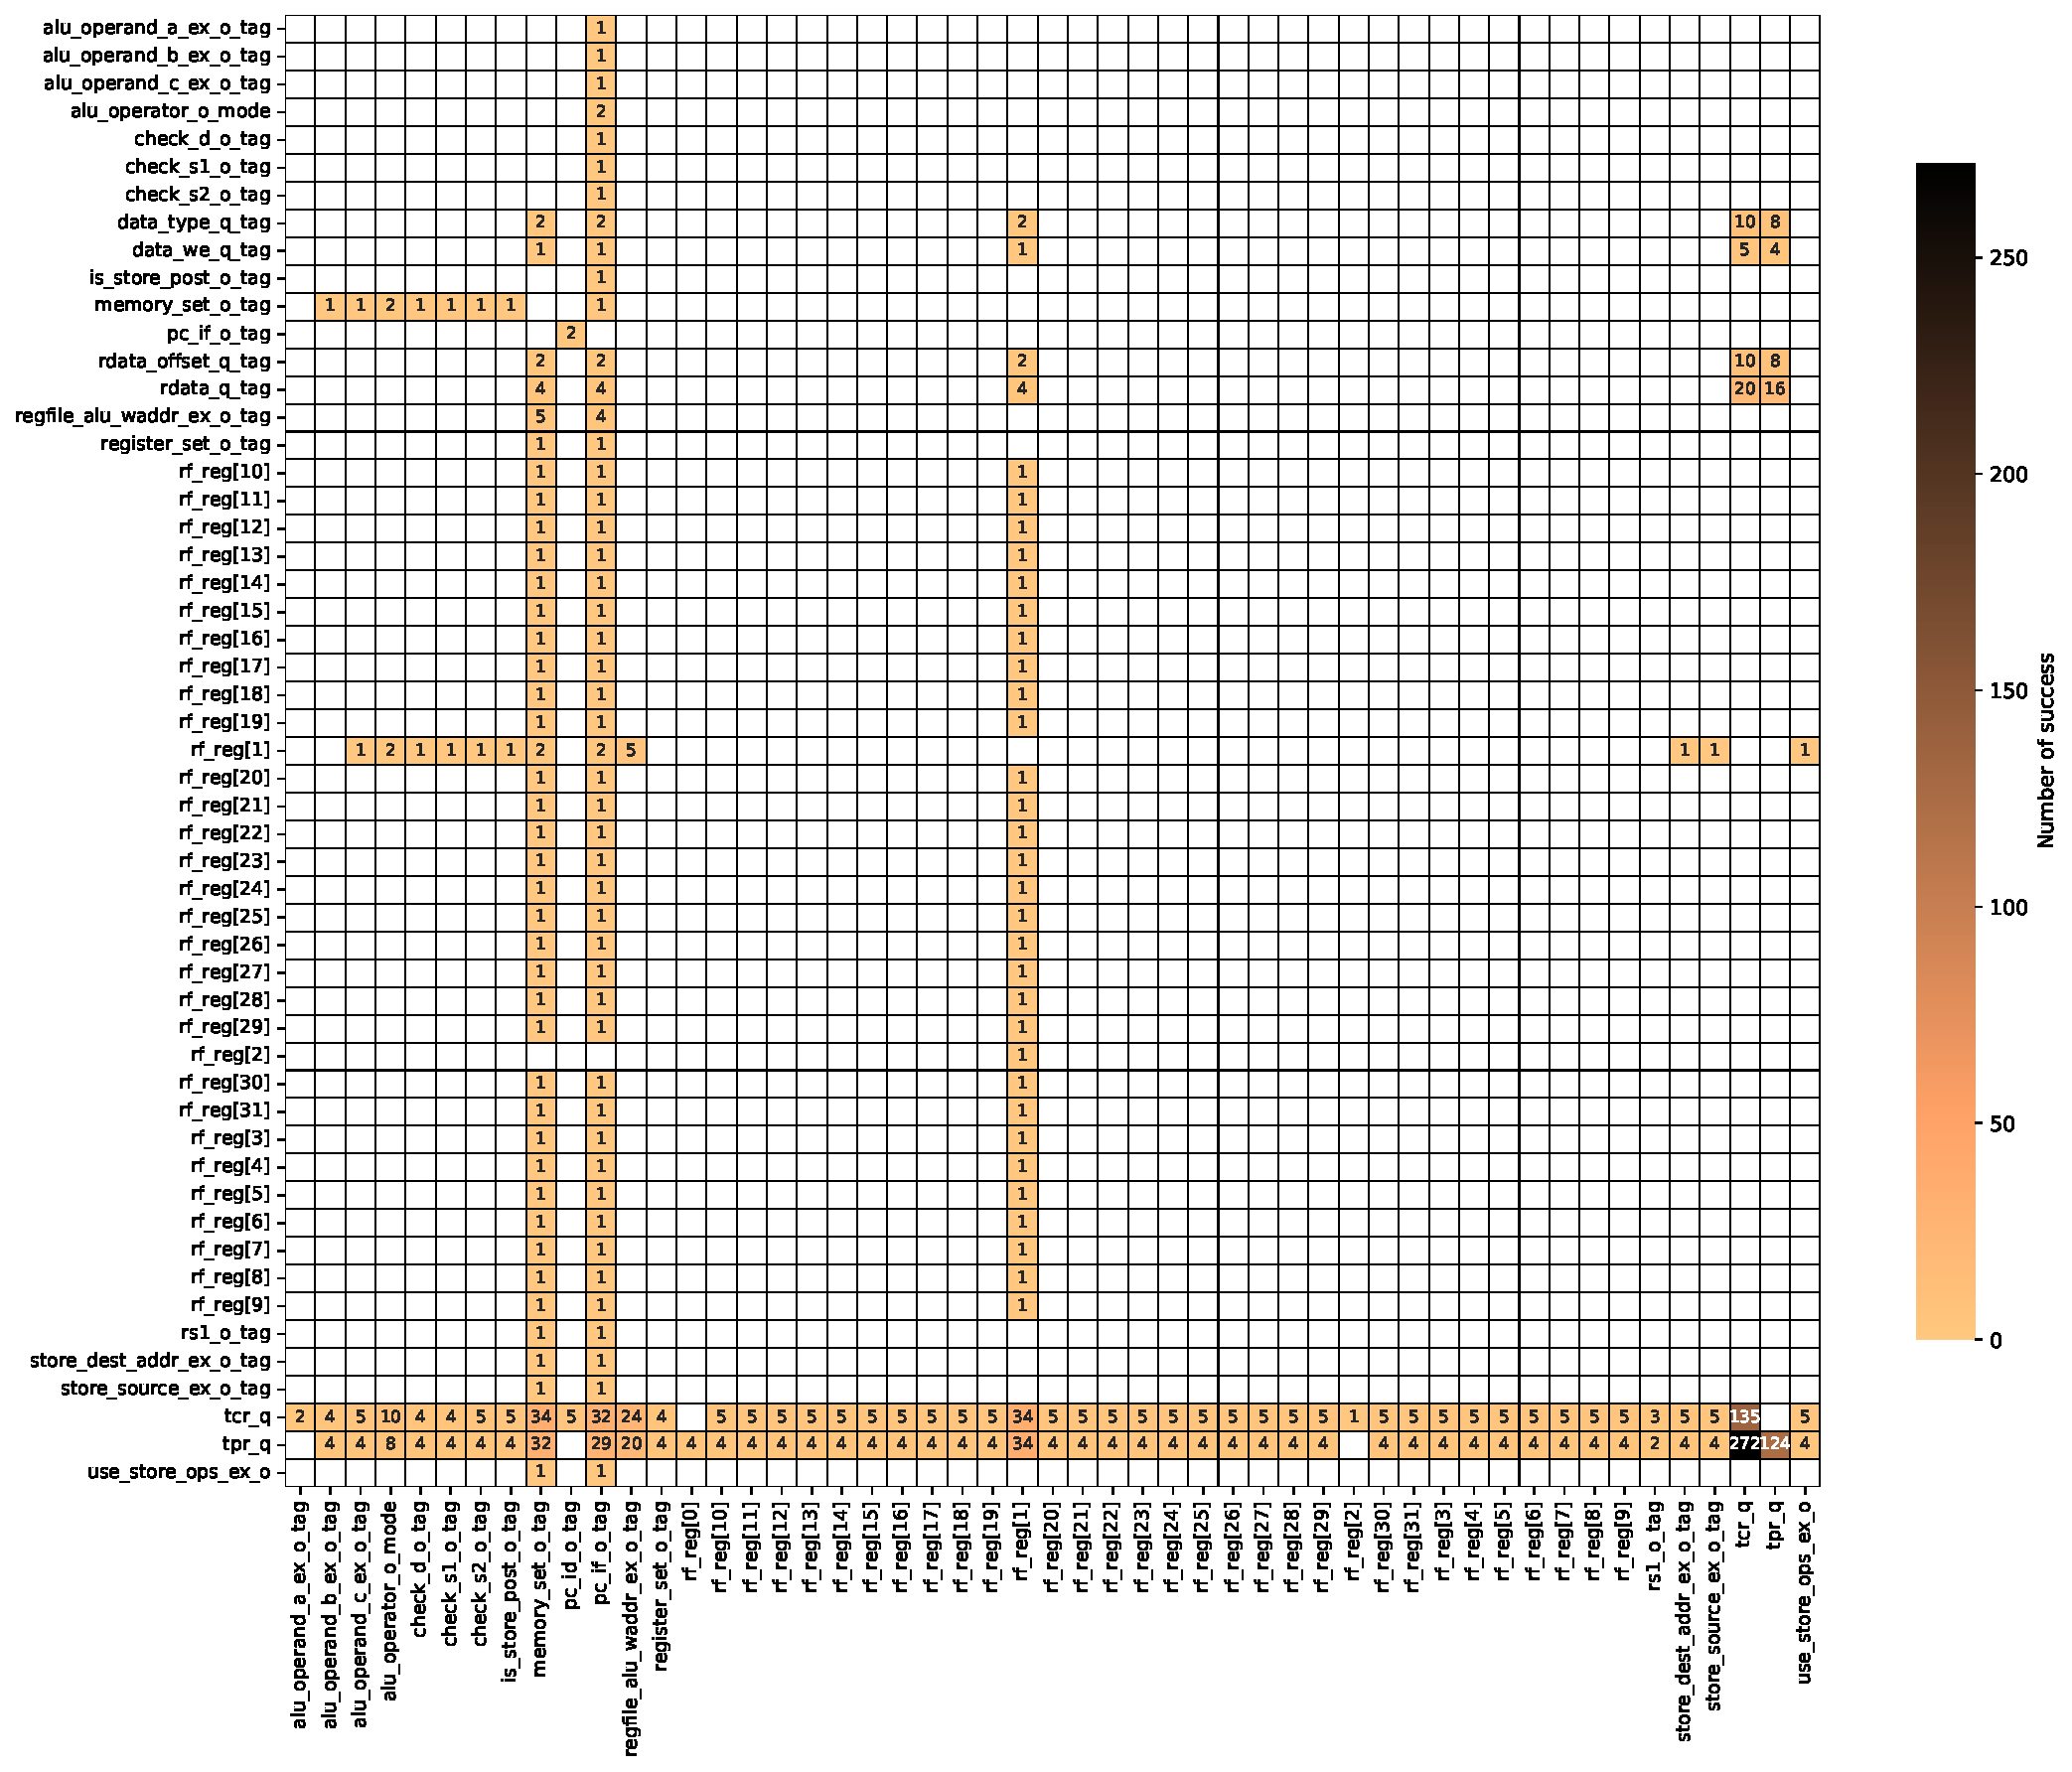
\includegraphics[width=\textwidth]{c6_group_composition/img/heatmap_buffer_overflow_wop_1_single_bitflip_spatial_2.pdf}
    \caption{Distribution of successes in the case of buffer overflow, unprotected, with a \textit{single bit-flip in two registers at a given clock cycle} fault model (1406 successes).}
    \label{fig:heatmap_bo_spatial_wop}
\end{figure}

\begin{figure}[ht]
    \centering
    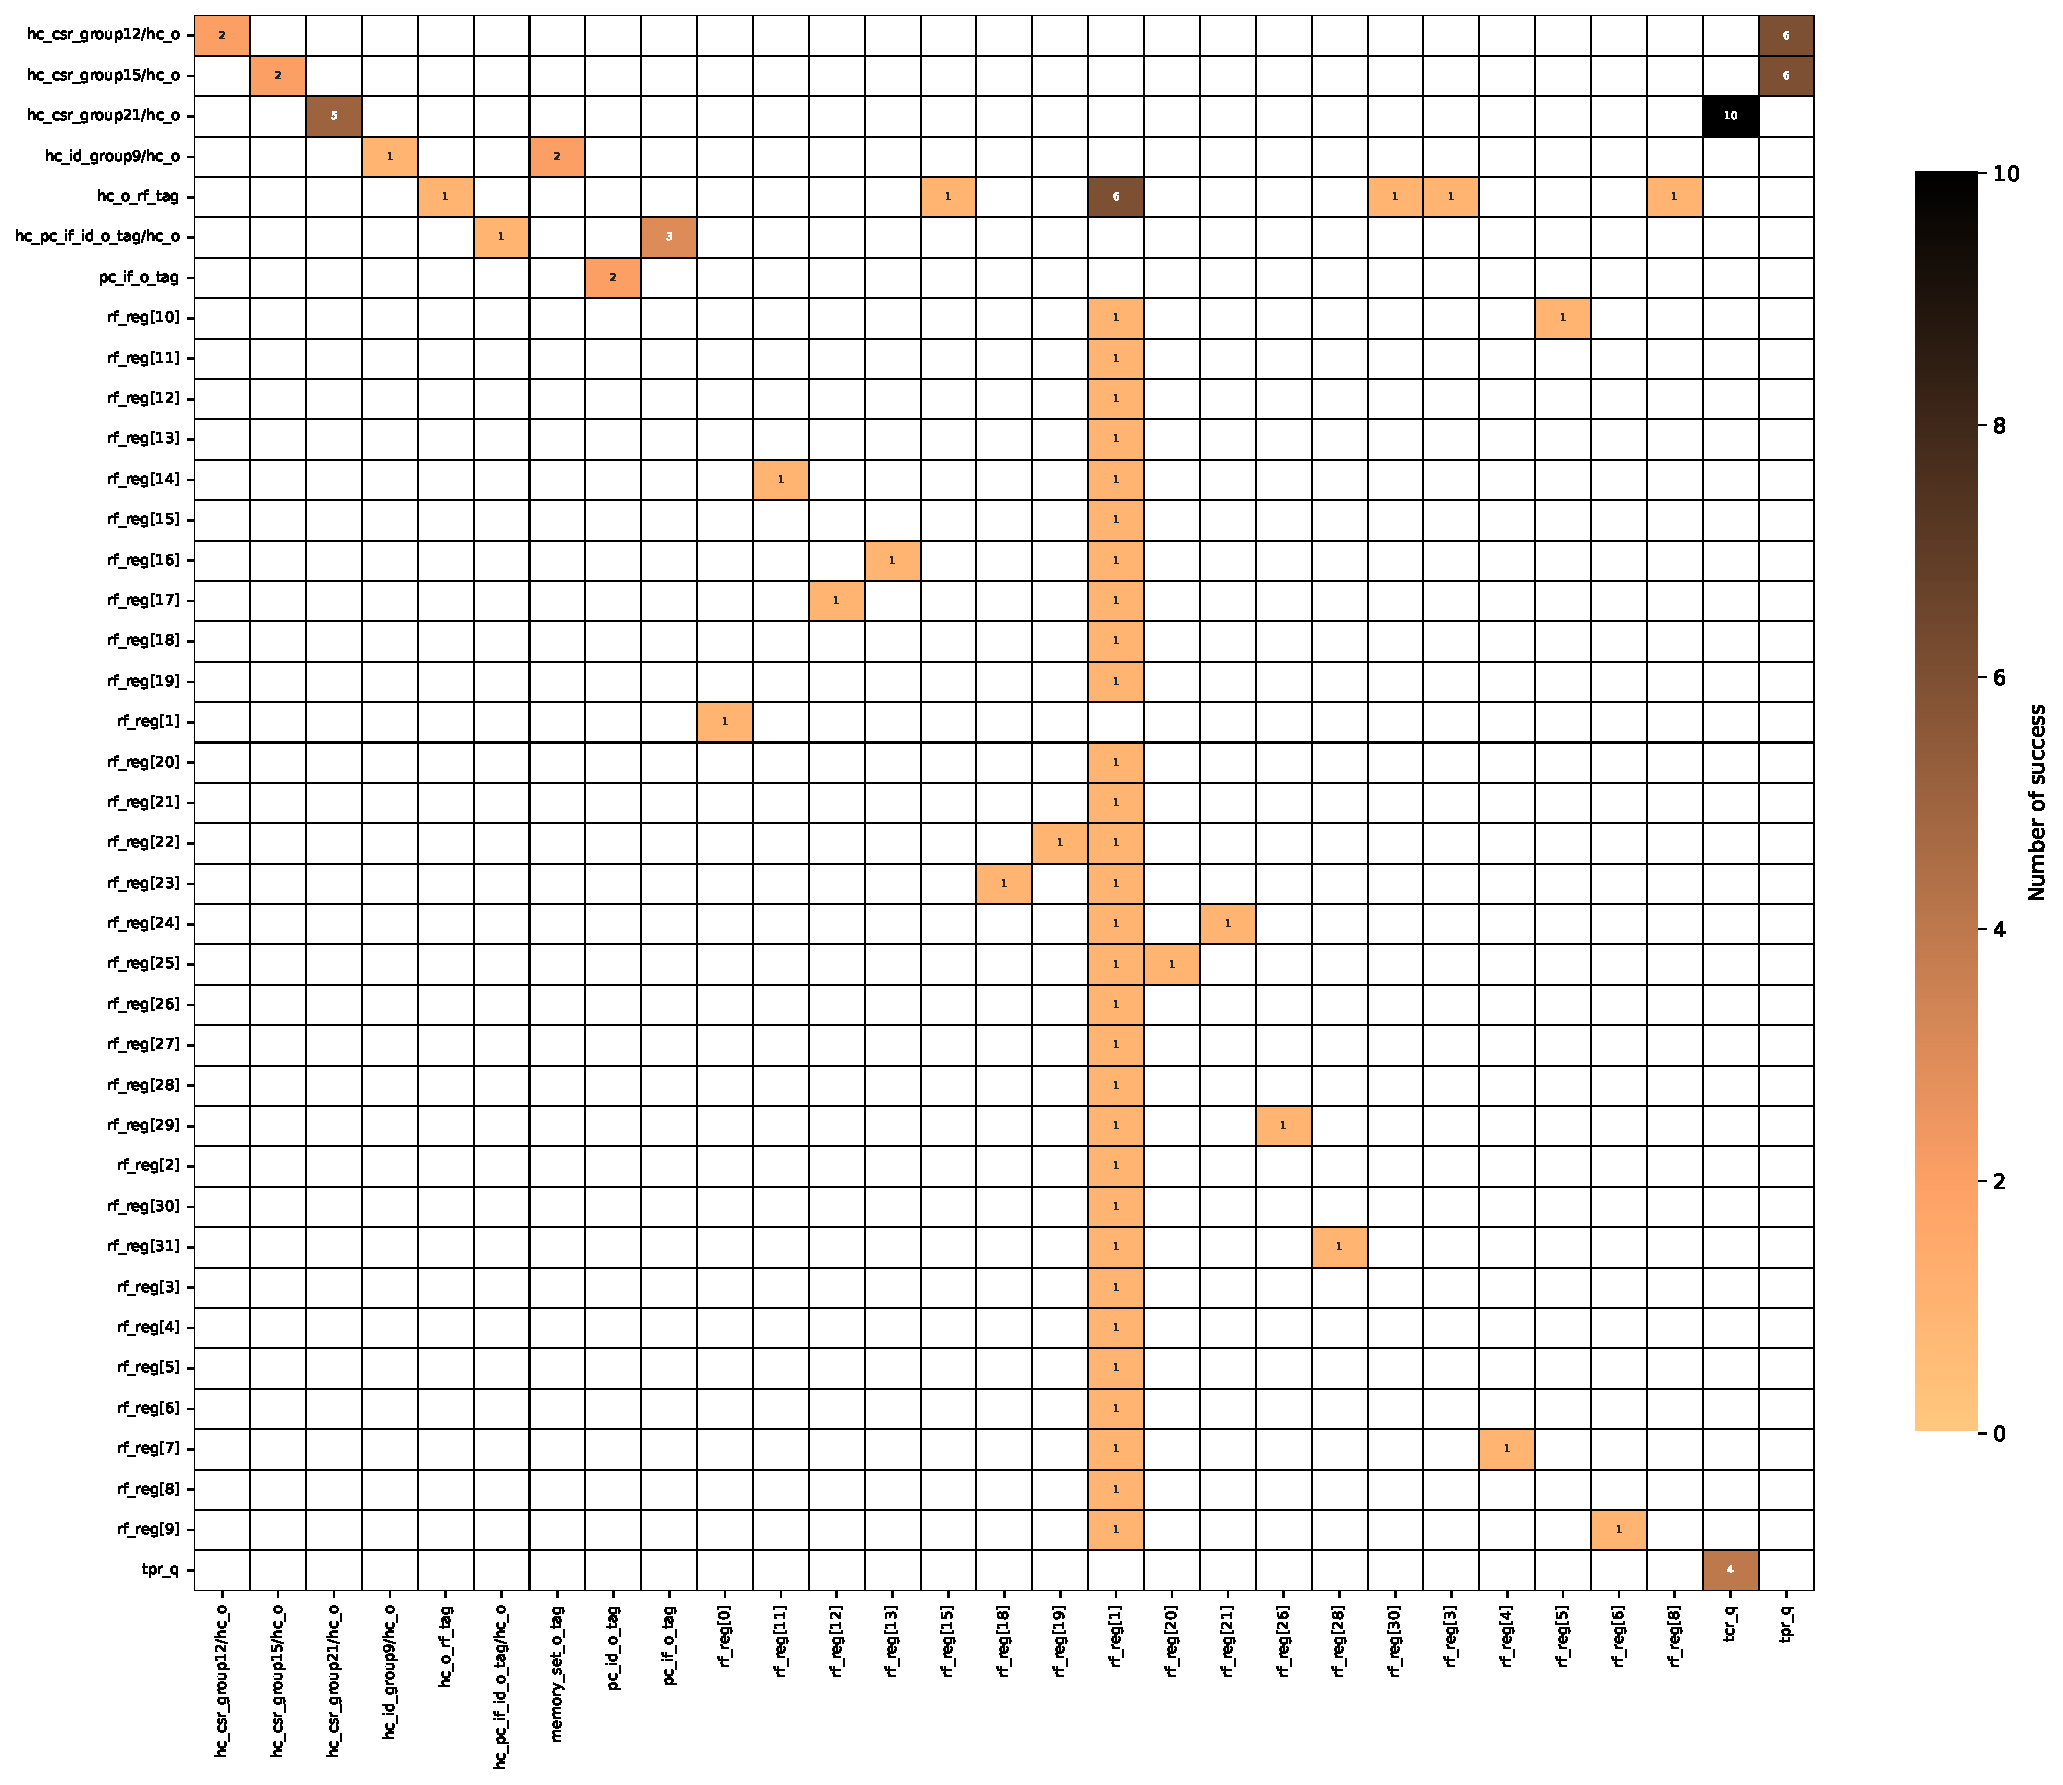
\includegraphics[width=\textwidth]{c6_group_composition/img/heatmap_buffer_overflow_hamming_5_single_bitflip_spatial_2.pdf}
    \caption{Distribution of successes in the case of buffer overflow, with the strategy 5 of Hamming Code, with a \textit{single bit-flip in two registers at a given clock cycle} fault model (98 successes).}
    \label{fig:heatmap_bo_spatial_hc5}
\end{figure}

\begin{figure}[ht]
    \centering
    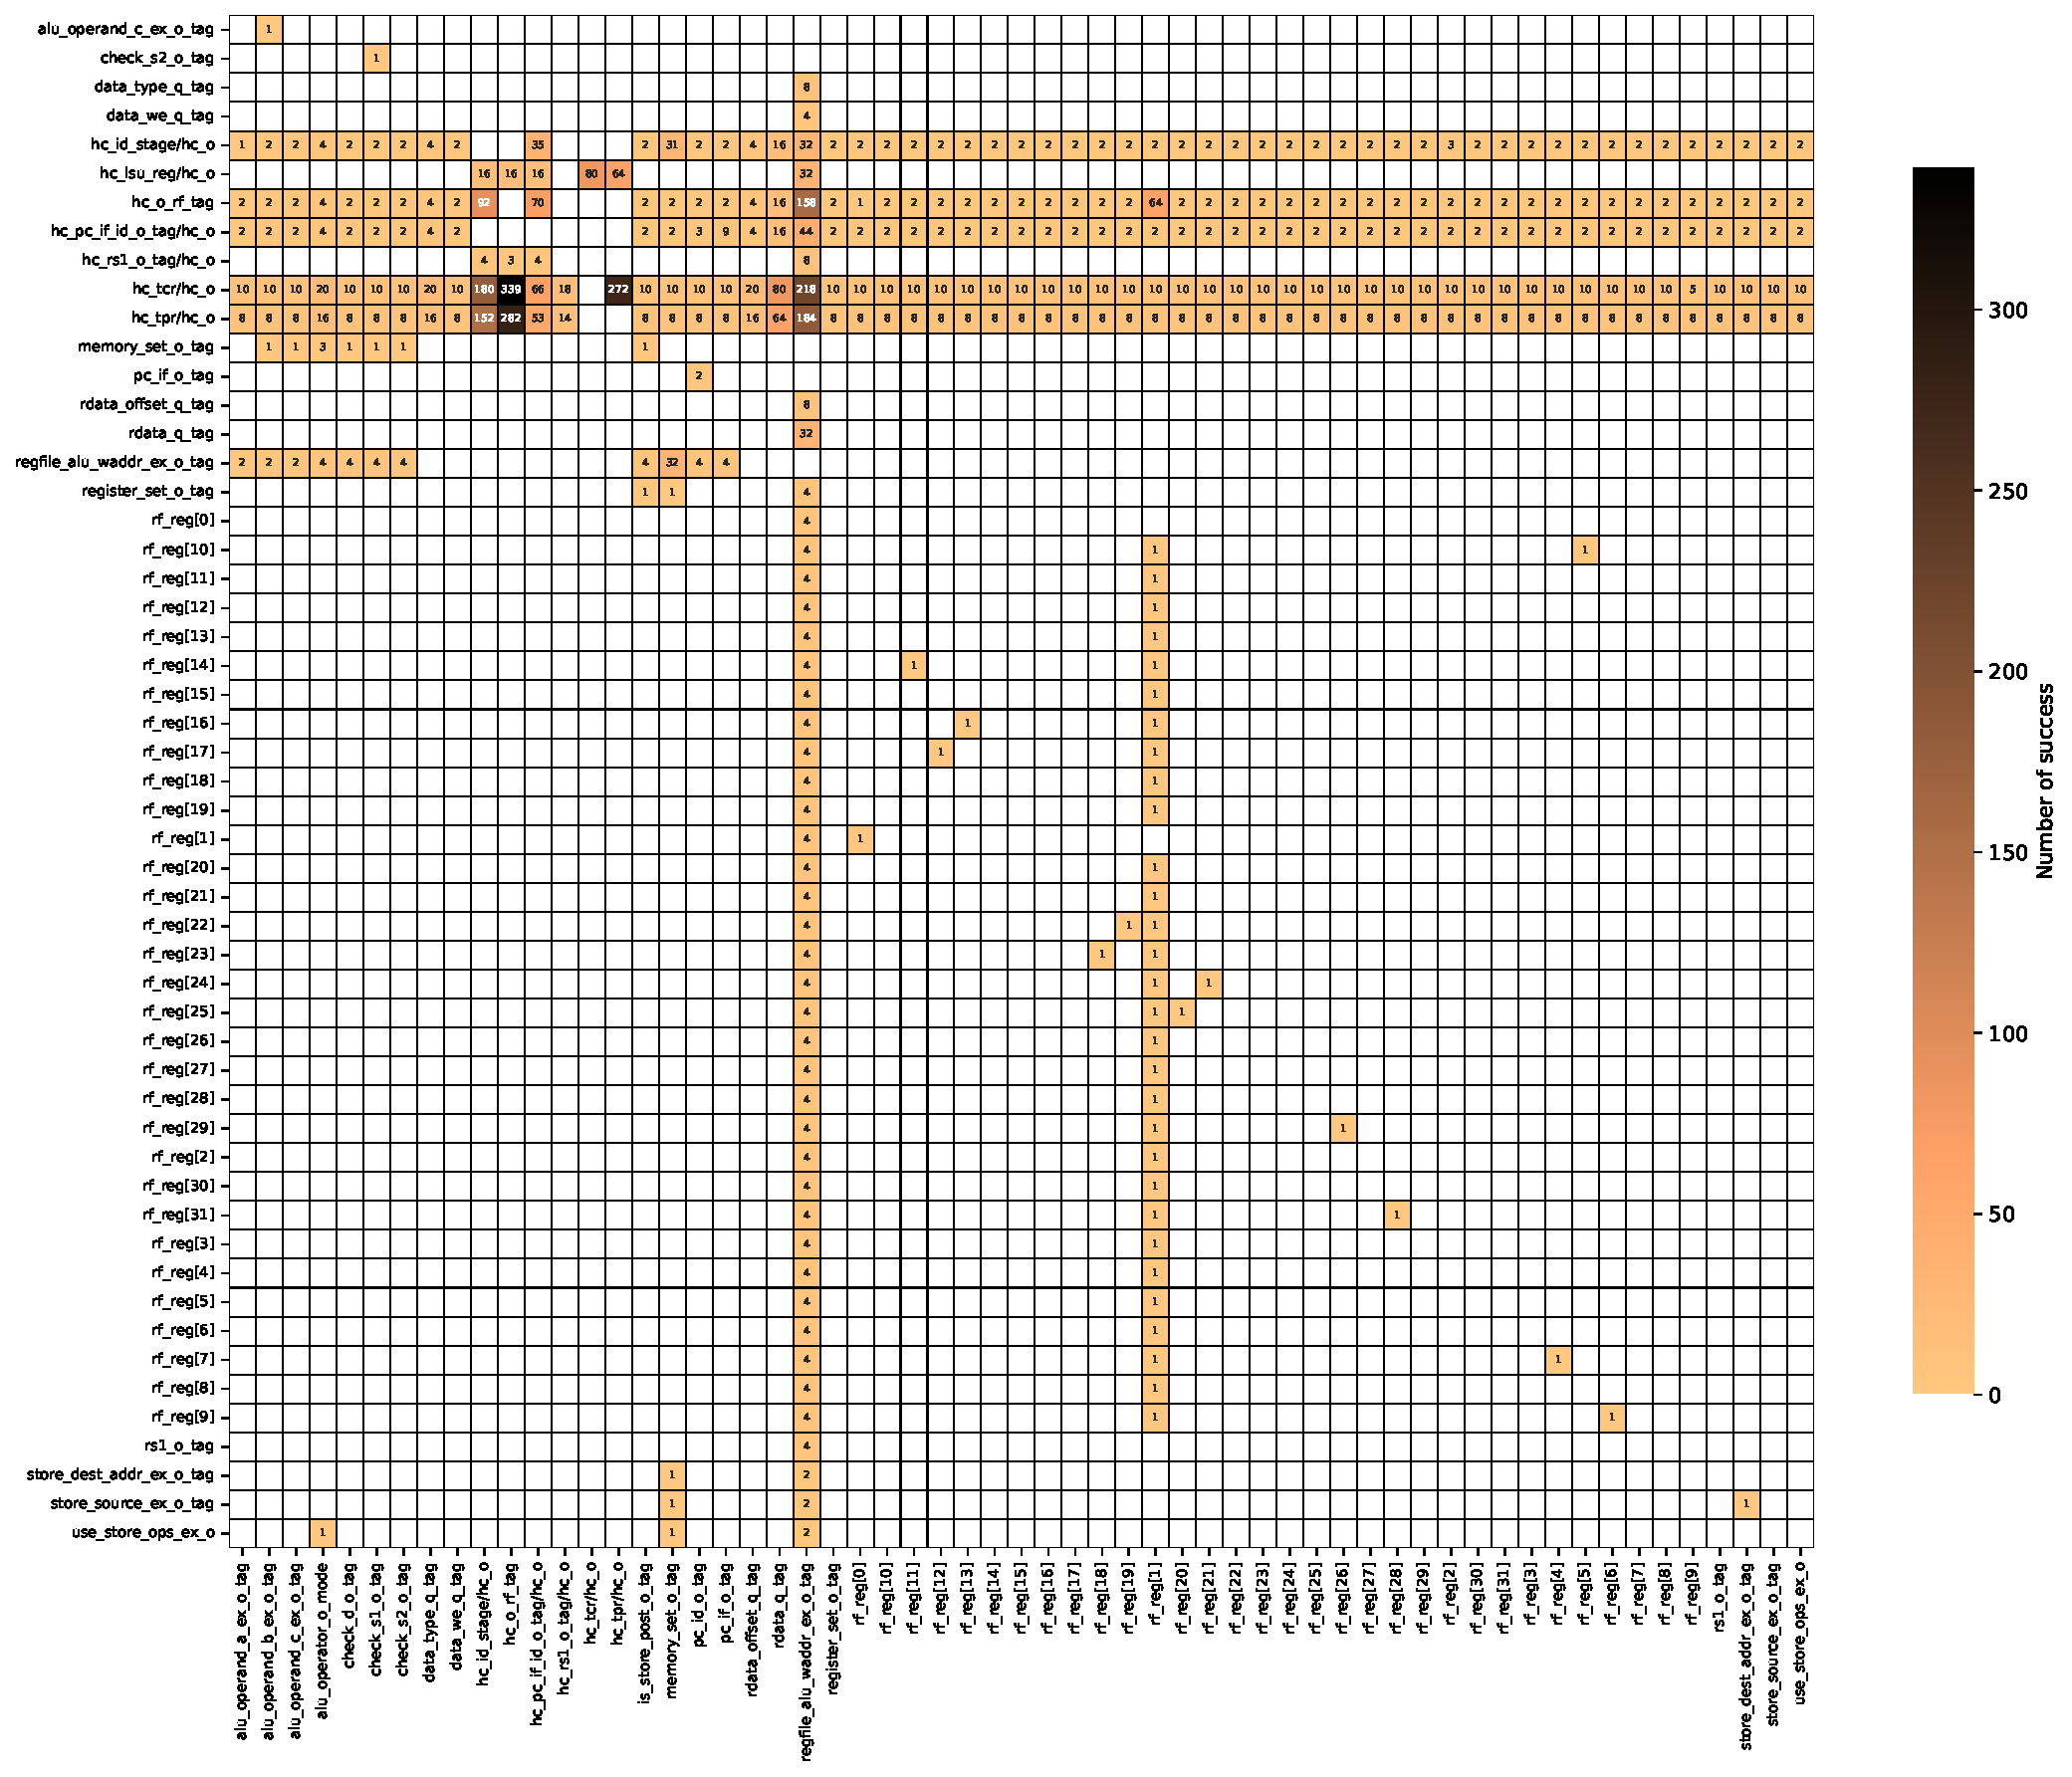
\includegraphics[width=.97\textwidth]{c6_group_composition/img/heatmap_buffer_overflow_hamming_2_multi_bitflip_reg_multi_2.pdf}
    \caption{Distribution of successes in the case of buffer overflow, with the 2nd strategy of Hamming Code, with \textit{multi-bit faults in two registers at a given clock cycle} fault model (4356 successes).}
    \label{fig:heatmap_bo_multireg_hc2}
\end{figure}

\begin{figure}[ht]
    \centering
    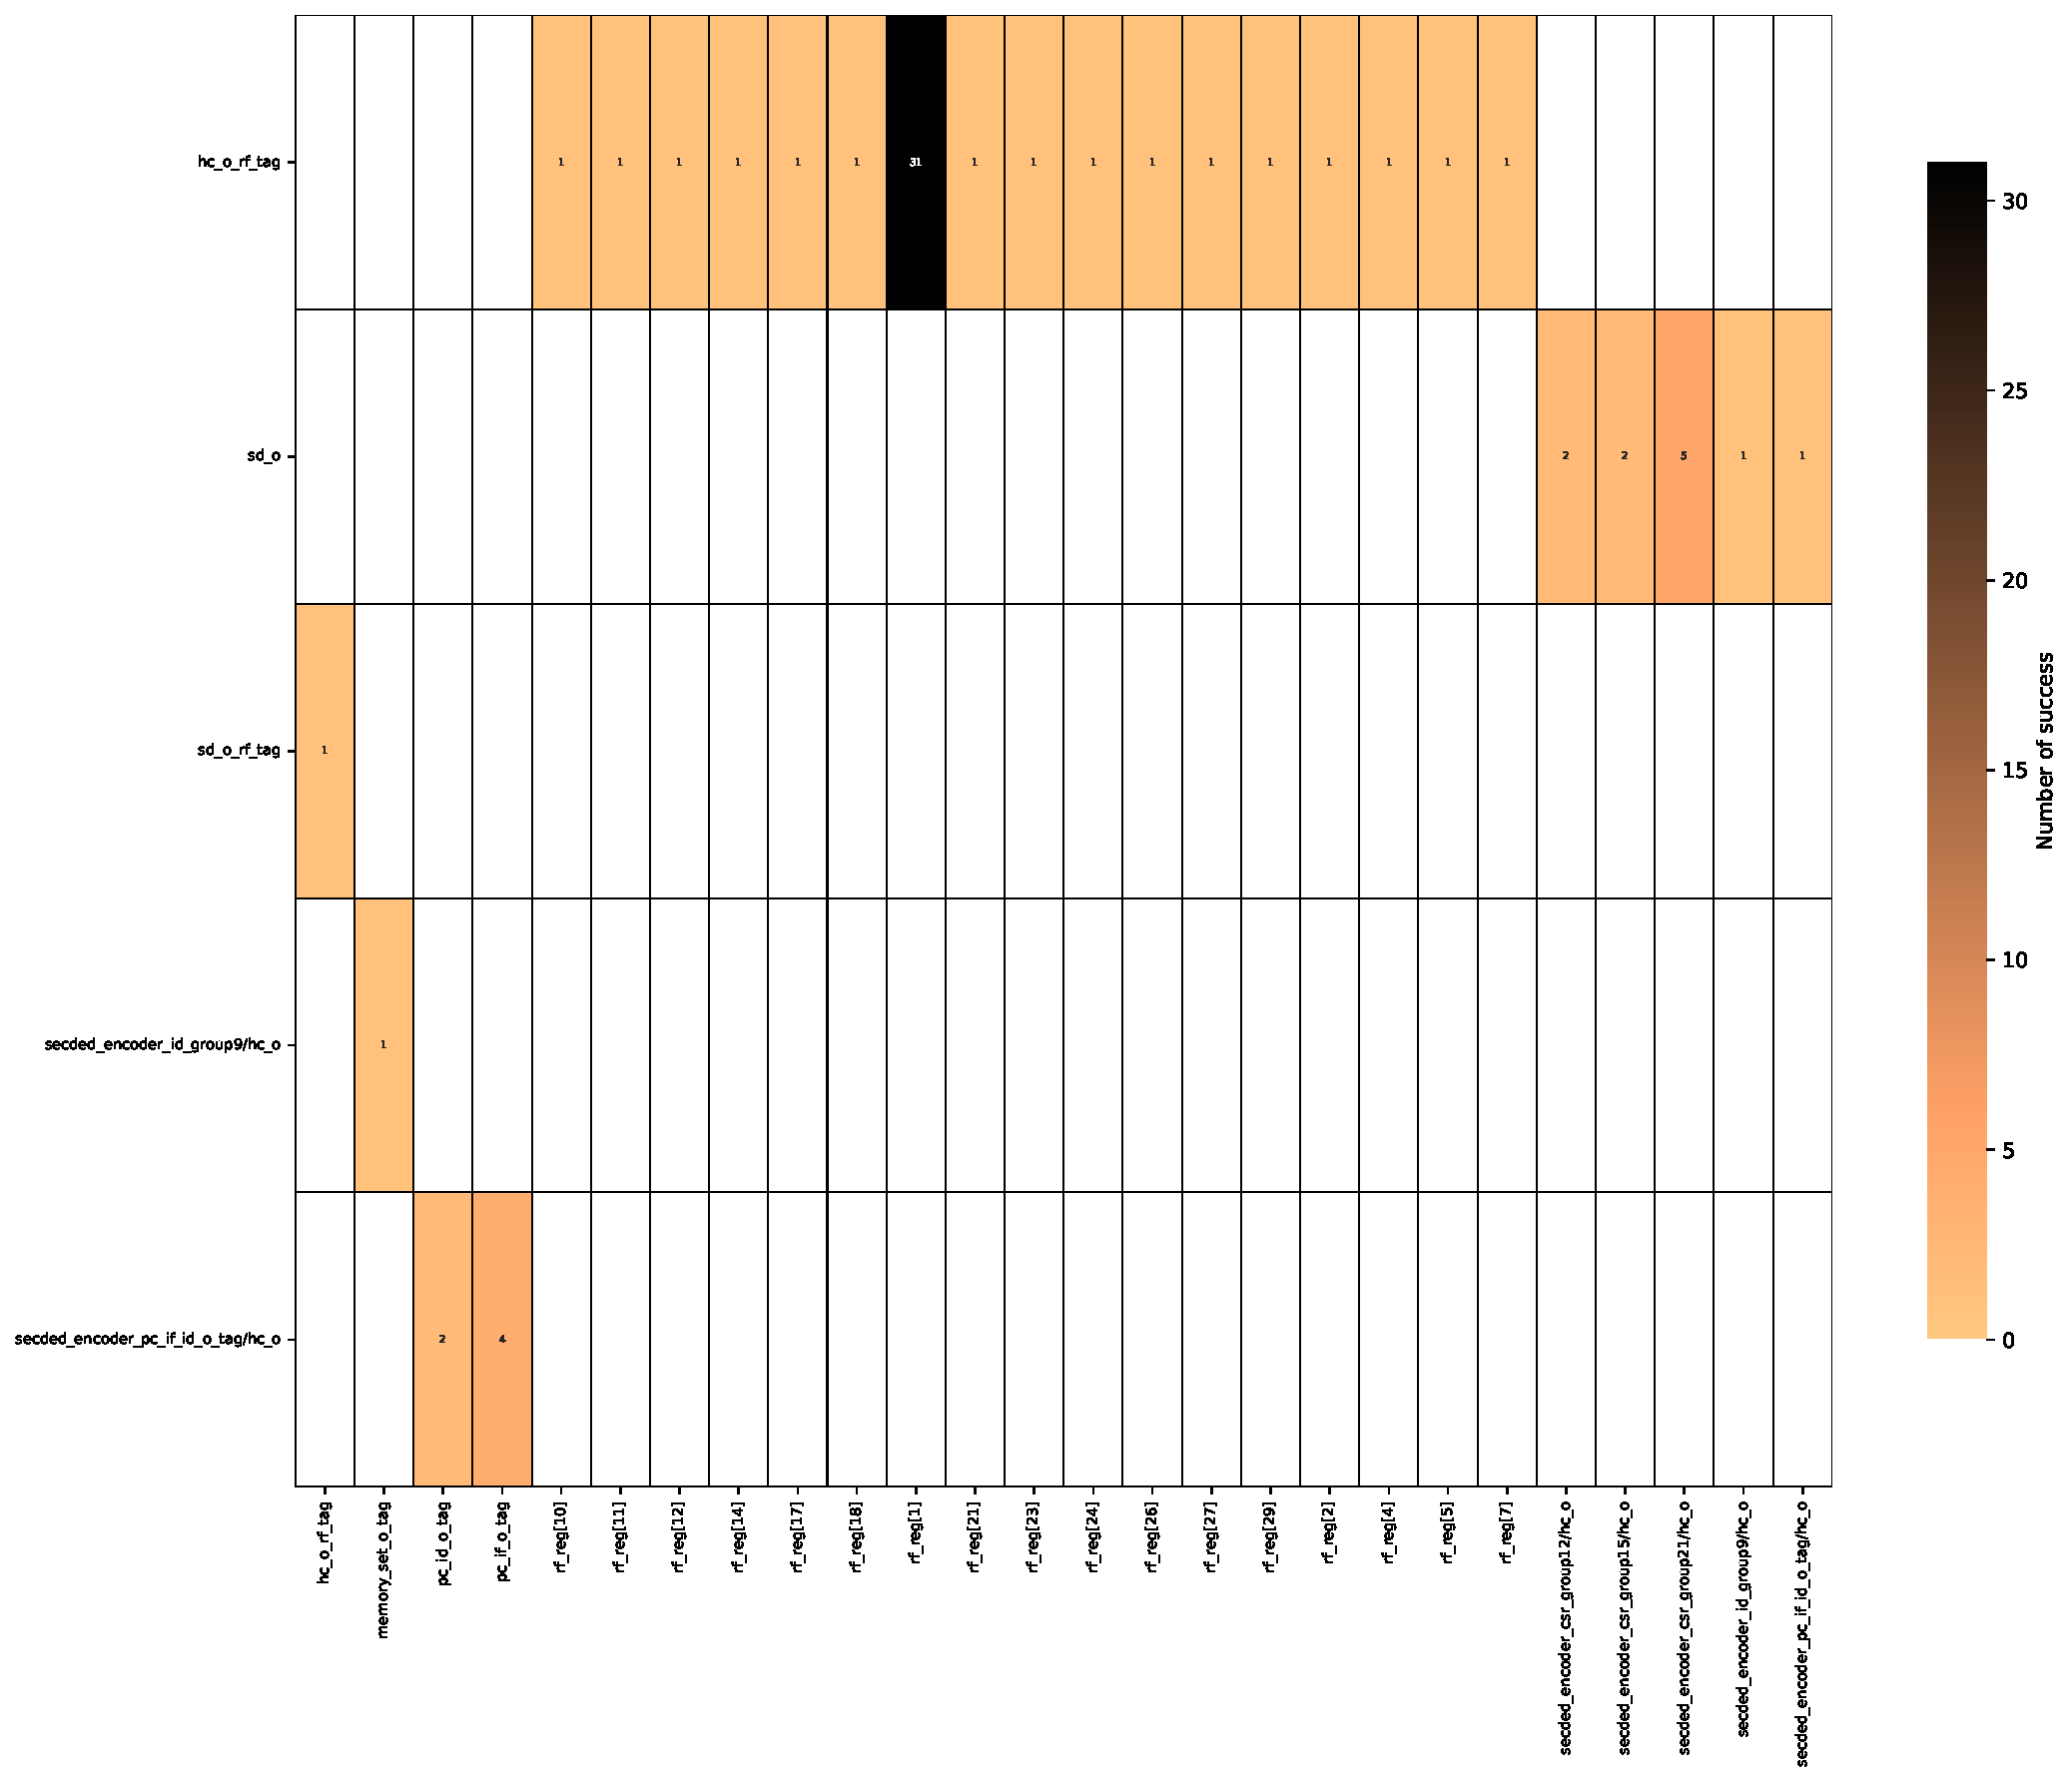
\includegraphics[width=\textwidth]{c6_group_composition/img/heatmap_buffer_overflow_secded_5_multi_bitflip_reg_multi_2.pdf}
    \caption{Distribution of successes in the case of buffer overflow, with the strategy 5 of SECDED, with \textit{multi-bit faults in two registers at a given clock cycle} fault model (66 successes).}
    \label{fig:heatmap_bo_multireg_sd5}
\end{figure}

In this subsection, we present our fault injection campaigns results targeting the DIFT-related registers of the D-RI5CY and its associated protection registers. We present one table for each fault model considered in this chapter containing the results for all the three use cases and all strategies (no protection, simple parity, Hamming Code 1 -- 5, and SECDED 1 -- 5).

Table~\ref{tab:chap6_results_single_bitflip_spatial} shows the results obtained from the \textit{single bit-flip in two registers at a given clock cycle} fault model according to each use case. This table shows that without any protection in the case of the buffer overflow, the D-RI5CY lead to 1406 successes with this fault model, while with the simple parity, we decrease from 1406 to 239 successes. However, due to the increase number of registers and the fact that Hamming Code can detect only one error, as we inject two faults, Hamming Code try to correct a fault but in many cases, it can cause a third fault increasing the number of successes. Nevertheless, the different proposed strategies decrease this number of successes by a factor of approximatively 50, going from 2.93\% to 0.06\%. The SECDED protection detect all injected faults thus no successes happen thanks to this countermeasure.
Table~\ref{tab:chap6_results_multi_bitflip_reg} shows the results obtained from the \textit{multi-bit faults in one register at a given clock cycle} fault model. This table depicts that Hamming Code induces more or less the same amount of fault than without any protection while simple parity shows better performances in terms of security. However, we can note a slight decrease for the second and third case. The best protection with Hamming Code is the fifth strategy as it shows the lower amount of successes. On the other hand, SECDED offers the best results in terms of protection, although it is not always successful against attacks depending on the strategy considered. For example, for the second use case, all five strategies led to some successes, whereas for the third use case, only the first strategy led to successes. As we are injecting multiple faults, up to 6 bit-flips, with this fault model, it is normal that there will still be some successes.
Table~\ref{tab:chap6_results_multi_bitflip_reg_multi} shows the results obtained from the \textit{multi-bit faults in two registers at a given clock cycle} fault model. This table represents the more complex fault model considered, for each use case and for each strategy there will be some successes. It is due to that fact that we can inject up to 12 faults in two registers even though SECDED can detect up to two faults. Hamming Code increase the number of successes depending on the strategy and the use case. However, if we just take into account the percentage, the different strategies allow to decrease with a significant factor the number of successes. For example, for the buffer overflow, the highest ratio of successes is due to the second strategy of Hamming Code at 1.33\% and the lowest ratio is thanks to the fifth strategy of SECDED at 0.0067\% (round to 0.01 in the table), which is approximatively 200 times less than 1.33\%.

\begin{table}[ht]
    \scriptsize
    \centering
    \caption{Logical fault injection simulation campaigns results for single bit-flip in two registers at a given clock cycle}
    \label{tab:chap6_results_single_bitflip_spatial}
    \setlength{\tabcolsep}{2pt}
    \begin{tabular}{@{}ccccccccccc@{}}
        \toprule
                                                           &                & Crash & Silent      & Delay      & Detection   & \tableTwoLines{Detection \&}{Correction} & \tableTwoLines{Double Error}{Detection} & Success                                              & Total         & \tableTwoLines{Execution}{time} \\\midrule
        \multirow{12}{*}{\tableTwoLines{Buffer}{Overflow}} & No protection  & 0     & \num{45097} & \num{1503} & --          & --                                       & --                                      & \num{1406} {\tiny (2.93\%)}                          & \num{48006}   & 13:43                           \\
                                                           & Simple parity  & 0     & \num{10551} & 134        & \num{40952} & --                                       & --                                      & 239 {\tiny (0.46\%)}                                 & \num{51876 }  & 14:07                           \\
                                                           & Hamming 1 & 0     & 0           & 575        & --          & \num{67829 }                             & --                                      & 452 {\tiny (0.66\%)}                                 & \num{68856 }  & 19:48                           \\
                                                           & Hamming 2 & 0     & 0           & 297        & --          & \num{72867 }                             & --                                      & 312 {\tiny (0.42\%)}                                 & \num{73476 }  & 97:16                           \\
                                                           & Hamming 3 & 0     & 0           & 263        & --          & \num{108326}                             & --                                      & 281 {\tiny (0.26\%)}                                 & \num{108870}  & 30:00                           \\
                                                           & Hamming 4 & 0     & 0           & 57         & --          & \num{155112}                             & --                                      & 99  {\tiny (0.06\%)}                                 & \num{155268}  & 46:30                           \\
                                                           & Hamming 5 & 0     & 0           & 55         & --          & \num{173367}                             & --                                      & 98  {\tiny (0.06\%)}                                 & \num{173520}  & 53:00                           \\
                                                           & SECDED 1       & 0     & 2436        & 0          & --          & \num{59424 }                             & \num{11616}                             & 0                                                    & \num{73476 }  & 20:56                           \\
                                                           & SECDED 2       & 0     & 0           & 0          & --          & \num{69354 }                             & \num{10842}                             & 0                                                    & \num{80196 }  & 21:49                           \\
                                                           & SECDED 3       & 0     & 0           & 0          & --          & \num{128376}                             & \num{9654 }                             & 0                                                    & \num{138030}  & 40:14                           \\
                                                           & SECDED 4       & 0     & 0           & 0          & --          & \num{204060}                             & \num{7410 }                             & 0                                                    & \num{211470}  & 64:02                           \\
                                                           & SECDED 5       & 0     & \num{12096} & 0          & --          & \num{214722}                             & \num{7542 }                             & 0                                                    & \num{234360}  & 69:44                           \\\midrule
        \multirow{12}{*}{\tableTwoLines{Format}{String}}   & No protection  & 0     & \num{55589} & \num{5035} & --          & --                                       & --                                      & \num{3384} {\tiny (5.29\%)}                          & \num{64008}   & 163:09                          \\
                                                           & Simple parity  & 0     & \num{13361} & 450        & \num{54590} & --                                       & --                                      & 767  {\tiny (1.11\%)}                                & \num{69168 }  & 114:06                          \\
                                                           & Hamming 1 & 0     & 0           & 1709       & --          & \num{89010 }                             & --                                      & 1089 {\tiny (1.19\%)}                                & \num{91808 }  & 179:38                          \\
                                                           & Hamming 2 & 0     & 0           & 982        & --          & \num{96182 }                             & --                                      & 804  {\tiny (0.82\%)}                                & \num{97968 }  & 136:40                          \\
                                                           & Hamming 3 & 0     & 0           & 659        & --          & \num{143883}                             & --                                      & 618  {\tiny (0.43\%)}                                & \num{145160}  & 261:40                          \\
                                                           & Hamming 4 & 0     & 0           & 379        & --          & \num{206423}                             & --                                      & 222  {\tiny (0.11\%)}                                & \num{207024}  & 368:10                          \\
                                                           & Hamming 5 & 0     & 0           & 391        & --          & \num{230758}                             & --                                      & 211  {\tiny (0.09\%)}                                & \num{231360}  & 445:58                          \\
                                                           & SECDED 1       & 0     & 0           & 0          & --          & \num{82480 }                             & \num{15488}                             & 0                                                    & \num{97968 }  & 233:28                          \\
                                                           & SECDED 2       & 0     & 0           & 0          & --          & \num{92472 }                             & \num{14456}                             & 0                                                    & \num{106928}  & 185:35                          \\
                                                           & SECDED 3       & 0     & 0           & 0          & --          & \num{171168}                             & \num{12872}                             & 0                                                    & \num{184040}  & 317:20                          \\
                                                           & SECDED 4       & 0     & 0           & 0          & --          & \num{272080}                             & \num{9880 }                             & 0                                                    & \num{281960}  & 462:58                          \\
                                                           & SECDED 5       & 0     & \num{16128} & 0          & --          & \num{286296}                             & \num{10056}                             & 0                                                    & \num{312480}  & 558:16                          \\\midrule
        \multirow{12}{*}{\tableTwoLines{Compare}{Compute}} & No protection  & 0     & \num{29906} & 919        & --          & --                                       & --                                      & \num{1179} {\tiny (3.68\%)}                          & \num{32004}   & 05:24                           \\
                                                           & Simple parity  & 0     & \num{6697}  & 202        & \num{27678} & --                                       & --                                      & 7   {\tiny (0.02\%)}                                 & \num{34584 }  & 04:48                           \\
                                                           & Hamming 1 & 0     & 0           & 450        & --          & \num{45192  }                            & --                                      & 262 {\tiny (0.57\%)}                                 & \num{45904 }  & 09:21                           \\
                                                           & Hamming 2 & 0     & 0           & 440        & --          & \num{48419  }                            & --                                      & 125 {\tiny (0.26\%)}                                 & \num{48984 }  & 08:47                           \\
                                                           & Hamming 3 & 0     & 0           & 315        & --          & \num{72140  }                            & --                                      & 125 {\tiny (0.17\%)}                                 & \num{72580 }  & 13:53                           \\
                                                           & Hamming 4 & 0     & 0           & 97         & --          & \num{103345 }                            & --                                      & 70  {\tiny (0.07\%)}                                 & \num{103512}  & 22:23                           \\
                                                           & Hamming 5 & 0     & 0           & 96         & --          & \num{115511 }                            & --                                      & 73  {\tiny (0.06\%)}                                 & \num{115680}  & 23:48                           \\
                                                           & SECDED 1       & 0     & 0           & 0          & --          & \num{37740  }                            & \num{11244}                             & 0                                                    & \num{48984 }  & 17:00                           \\
                                                           & SECDED 2       & 0     & 0           & 0          & --          & \num{46236  }                            & \num{7228}                              & 0                                                    & \num{53464 }  & 10:12                           \\
                                                           & SECDED 3       & 0     & 0           & 0          & --          & \num{85584  }                            & \num{6436}                              & 0                                                    & \num{92020 }  & 18:25                           \\
                                                           & SECDED 4       & 0     & 0           & 0          & --          & \num{136040 }                            & \num{4940}                              & 0                                                    & \num{140980}  & 28:37                           \\
                                                           & SECDED 5       & 0     & 0           & 0          & --          & \num{151212 }                            & \num{5028}                              & 0                                                    & \num{156240}  & 32:52                           \\\midrule
        Total                                              &                &       &             &            &             &                                          &                                         & \num{11823} {\tiny (\compute{11823*100/4252212}{2})} & \num{4252212} &                                 \\
        \bottomrule
    \end{tabular}
\end{table}

\begin{table}[ht]
    \scriptsize
    \centering
    \caption{Logical fault injection simulation campaigns results for exhaustive multi-bits faults in one register at a given clock cycle}
    \label{tab:chap6_results_multi_bitflip_reg}
    \setlength{\tabcolsep}{3pt}
    \begin{tabular}{@{}ccccccccccc@{}}
        \toprule
                                                           &                & Crash & Silent & Delay & Detection & \tableTwoLines{Detection \&}{Correction} & \tableTwoLines{Double Error}{Detection} & Success                                       & Total       & \tableTwoLines{Execution}{time} \\\midrule
        \multirow{12}{*}{\tableTwoLines{Buffer}{Overflow}} & No protection  & 0     & 927    & 6     & --        & --                                       & --                                      & 3 {\tiny (0.32\%)}                            & 936         & 00:08                           \\
                                                           & Simple parity  & 0     & 498    & 0     & 498       & --                                       & --                                      & 0                                             & 996         & 00:14                           \\
                                                           & Hamming 1 & 0     & 0      & 20    & --        & 1962                                     & --                                      & 10 {\tiny (0.50\%)}                           & 1992        & 00:28                           \\
                                                           & Hamming 2 & 0     & 0      & 12    & --        & 2038                                     & --                                      & 14 {\tiny (0.68\%)}                           & 2064        & 00:32                           \\
                                                           & Hamming 3 & 0     & 0      & 12    & --        & 2352                                     & --                                      & 12 {\tiny (0.51\%)}                           & 2376        & 00:28                           \\
                                                           & Hamming 4 & 0     & 0      & 12    & --        & 2712                                     & --                                      & 12 {\tiny (0.44\%)}                           & 2736        & 00:35                           \\
                                                           & Hamming 5 & 0     & 0      & 12    & --        & 2976                                     & --                                      & 12 {\tiny (0.40\%)}                           & 3000        & 00:45                           \\
                                                           & SECDED 1       & 0     & 0      & 8     & --        & 1393                                     & 648                                     & 3 {\tiny (0.15\%)}                            & 2052        & 00:30                           \\
                                                           & SECDED 2       & 0     & 0      & 5     & --        & 1475                                     & 666                                     & 2 {\tiny (0.09\%)}                            & 2148        & 00:30                           \\
                                                           & SECDED 3       & 0     & 0      & 4     & --        & 1932                                     & 726                                     & 2 {\tiny (0.08\%)}                            & 2664        & 00:40                           \\
                                                           & SECDED 4       & 0     & 0      & 0     & --        & 2370                                     & 822                                     & 0                                             & 3192        & 00:45                           \\
                                                           & SECDED 5       & 0     & 0      & 0     & --        & 2670                                     & 798                                     & 0                                             & 3468        & 00:55                           \\\midrule
        \multirow{12}{*}{\tableTwoLines{Format}{String}}   & No protection  & 0     & 1202   & 32    & --        & --                                       & --                                      & 14 {\tiny (1.12\%)}                           & 1248        & 01:24                           \\
                                                           & Simple parity  & 0     & 661    & 0     & 665       & --                                       & --                                      & 2  {\tiny (0.15\%)}                           & 1328        & 02:12                           \\
                                                           & Hamming 1 & 0     & 0      & 62    & --        & 2565                                     & --                                      & 29 {\tiny (1.09\%)}                           & 2656        & 04:24                           \\
                                                           & Hamming 2 & 0     & 0      & 53    & --        & 2666                                     & --                                      & 33 {\tiny (1.20\%)}                           & 2752        & 03:36                           \\
                                                           & Hamming 3 & 0     & 0      & 47    & --        & 3090                                     & --                                      & 31 {\tiny (0.98\%)}                           & 3168        & 03:55                           \\
                                                           & Hamming 4 & 0     & 0      & 47    & --        & 3570                                     & --                                      & 31 {\tiny (0.85\%)}                           & 3648        & 04:25                           \\
                                                           & Hamming 5 & 0     & 0      & 41    & --        & 3930                                     & --                                      & 29 {\tiny (0.73\%)}                           & 4000        & 05:18                           \\
                                                           & SECDED 1       & 0     & 0      & 22    & --        & 1832                                     & 864                                     & 18 {\tiny (0.66\%)}                           & 2736        & 03:30                           \\
                                                           & SECDED 2       & 0     & 0      & 14    & --        & 1938                                     & 894                                     & 18 {\tiny (0.63\%)}                           & 2864        & 03:48                           \\
                                                           & SECDED 3       & 0     & 0      & 10    & --        & 2560                                     & 968                                     & 14 {\tiny (0.39\%)}                           & 3552        & 04:42                           \\
                                                           & SECDED 4       & 0     & 0      & 5     & --        & 3146                                     & 1096                                    & 9  {\tiny (0.21\%)}                           & 4256        & 05:42                           \\
                                                           & SECDED 5       & 0     & 0      & 4     & --        & 3554                                     & 1064                                    & 2  {\tiny (0.04\%)}                           & 4624        & 06:30                           \\\midrule
        \multirow{12}{*}{\tableTwoLines{Compare}{Compute}} & No protection  & 0     & 616    & 2     & --        & --                                       & --                                      & 6  {\tiny (0.96\%)}                           & 624         & 00:04                           \\
                                                           & Simple parity  & 0     & 330    & 0     & 334       & --                                       & --                                      & 0                                             & 664         & 00:04                           \\
                                                           & Hamming 1 & 0     & 0      & 9     & --        & 1311                                     & --                                      & 8 {\tiny (0.60\%)}                            & 1328        & 00:09                           \\
                                                           & Hamming 2 & 0     & 0      & 15    & --        & 1356                                     & --                                      & 5 {\tiny (0.36\%)}                            & 1376        & 00:09                           \\
                                                           & Hamming 3 & 0     & 0      & 12    & --        & 1567                                     & --                                      & 5 {\tiny (0.32\%)}                            & 1584        & 00:11                           \\
                                                           & Hamming 4 & 0     & 0      & 12    & --        & 1807                                     & --                                      & 5 {\tiny (0.27\%)}                            & 1824        & 00:13                           \\
                                                           & Hamming 5 & 0     & 0      & 12    & --        & 1983                                     & --                                      & 5 {\tiny (0.25\%)}                            & 2000        & 00:14                           \\
                                                           & SECDED 1       & 0     & 0      & 2     & --        & 888                                      & 476                                     & 2 {\tiny (0.15\%)}                            & 1368        & 00:09                           \\
                                                           & SECDED 2       & 0     & 0      & 6     & --        & 977                                      & 449                                     & 0                                             & 1432        & 00:10                           \\
                                                           & SECDED 3       & 0     & 0      & 2     & --        & 1290                                     & 484                                     & 0                                             & 1776        & 00:12                           \\
                                                           & SECDED 4       & 0     & 0      & 0     & --        & 1580                                     & 548                                     & 0                                             & 2128        & 00:15                           \\
                                                           & SECDED 5       & 0     & 0      & 0     & --        & 1780                                     & 532                                     & 0                                             & 2312        & 00:16                           \\\midrule
        Total                                              &                &       &        &       &           &                                          &                                         & \num{336} {\tiny(\compute{336*100/82872}{2})} & \num{82872} &                                 \\
        \bottomrule
    \end{tabular}
\end{table}

\begin{table}[ht]
    \scriptsize
    \centering
    \caption{Logical fault injection simulation campaigns results for exhaustive multi-bits faults in two registers at a given clock cycle}
    \label{tab:chap6_results_multi_bitflip_reg_multi}
    \setlength{\tabcolsep}{1pt}
    \begin{tabular}{@{}ccccccccccc@{}}
        \toprule
                                                           &               & Crash & Silent       & Delay       & Detection   & \tableTwoLines{Detection \&}{Correction} & \tableTwoLines{Double Error}{Detection} & Success                      & Total          & \tableTwoLines{Execution}{time} \\\midrule
        \multirow{12}{*}{\tableTwoLines{Buffer}{Overflow}} & No protection & 0     & \num{67072 } & 926         & --          & --                                       & --                                      & 450 {\tiny (0.66\%)}         & \num{68448 }   & 11:11                           \\
                                                           & Simple parity & 0     & \num{24622 } & 8           & \num{53359} & --                                       & --                                      & 59 {\tiny (0.08\%)}          & \num{78048 }   & 25:00                           \\
                                                           & Hamming 1     & 0     & \num{294464} & 6273        & --          & --                                       & --                                      & 3103 {\tiny (1.02\%)}        & \num{303840}   & 99:36                           \\
                                                           & Hamming 2     & 0     & 0            & 3992        & --          & \num{319588}                             & --                                      & 4356 {\tiny (1.33\%)}        & \num{327936}   & 131:12                          \\
                                                           & Hamming 3     & 0     & 0            & 4557        & --          & \num{436187}                             & --                                      & 4408 {\tiny (0.99\%)}        & \num{445152}   & 121:20                          \\
                                                           & Hamming 4     & 0     & 0            & 5446        & --          & \num{590953}                             & --                                      & 5329 {\tiny (0.89\%)}        & \num{601728}   & 167:00                          \\
                                                           & Hamming 5     & 0     & 0            & 5987        & --          & \num{714873}                             & --                                      & 5860 {\tiny (0.81\%)}        & \num{726720}   & 210:31                          \\
                                                           & SECDED 1      & 0     & 0            & 1911        & --          & \num{150791}                             & \num{170575}                            & 723 {\tiny (0.22\%)}         & \num{324000}   & 86:59                           \\
                                                           & SECDED 2      & 0     & 0            & 1186        & --          & \num{170805}                             & \num{184761}                            & 584 {\tiny (0.16\%)}         & \num{357336}   & 94:04                           \\
                                                           & SECDED 3      & 0     & 0            & 1230        & --          & \num{300260}                             & \num{263665}                            & 669 {\tiny (0.12\%)}         & \num{565824}   & 161:30                          \\
                                                           & SECDED 4      & 0     & 0            & 18          & --          & \num{457498}                             & \num{368959}                            & 61 {\tiny (0.01\%)}          & \num{826536}   & 244:48                          \\
                                                           & SECDED 5      & 0     & 0            & 39          & --          & \num{576992}                             & \num{401407}                            & 66 {\tiny (0.01\%)}          & \num{978504}   & 284:45                          \\\midrule
        \multirow{12}{*}{\tableTwoLines{Format}{String}}   & No protection & 0     & \num{84419}  & 4836        & --          & --                                       & --                                      & 2009 {\tiny (2.20\%)}        & \num{91264 }   & 104:15                          \\
                                                           & Simple parity & 0     & \num{32275}  & 147         & \num{71198} & --                                       & --                                      & 444 {\tiny (0.43\%)}         & \num{104064}   & 138:40                          \\
                                                           & Hamming 1     & 0     & 0            & \num{20050} & --          & \num{375836}                             & --                                      & 9234 {\tiny (2.28\%)}        & \num{405120}   & 902:08                          \\
                                                           & Hamming 2     & 0     & 0            & \num{17597} & --          & \num{408894}                             & --                                      & \num{10757} {\tiny (2.46\%)} & \num{437248}   & 774:40                          \\
                                                           & Hamming 3     & 0     & 0            & \num{17926} & --          & \num{564154}                             & --                                      & \num{11456} {\tiny (1.93\%)} & \num{593536}   & 1021:50                         \\
                                                           & Hamming 4     & 0     & 0            & \num{20986} & --          & \num{767604}                             & --                                      & \num{13714} {\tiny (1.71\%)} & \num{802304}   & 1418:24                         \\
                                                           & Hamming 5     & 0     & 0            & \num{20547} & --          & \num{934077}                             & --                                      & \num{14336} {\tiny (1.48\%)} & \num{968960}   & 1690:05                         \\
                                                           & SECDED 1      & 0     & 0            & 5408        & --          & \num{194766}                             & \num{227655}                            & 4171 {\tiny (0.97\%)}        & \num{432000}   & 740:21                          \\
                                                           & SECDED 2      & 0     & 0            & 3611        & --          & \num{220568}                             & \num{247704}                            & 4565 {\tiny (0.96\%)}        & \num{476448}   & 836:41                          \\
                                                           & SECDED 3      & 0     & 0            & 3088        & --          & \num{395487}                             & \num{351553}                            & 4304 {\tiny (0.57\%)}        & \num{754432}   & 1305:36                         \\
                                                           & SECDED 4      & 0     & 0            & 1939        & --          & \num{604649}                             & \num{491945}                            & 3515 {\tiny (0.32\%)}        & \num{1102048}  & 1915:20                         \\
                                                           & SECDED 5      & 0     & 0            & 1938        & --          & \num{766527}                             & \num{535209}                            & 998 {\tiny (0.08\%)}         & \num{1304672}  & 2287:38                         \\\midrule
        \multirow{12}{*}{\tableTwoLines{Compare}{Compute}} & No protection & 0     & \num{44444}  & 323         & --          & --                                       & --                                      & 865 {\tiny (1.90\%)}         & \num{45632 }   & 05:36                           \\
                                                           & Simple parity & 0     & \num{16033}  & 53          & \num{35943} & --                                       & --                                      & 3 {\tiny (0.01\%)}           & \num{52032 }   & 08:05                           \\
                                                           & Hamming 1     & 0     & 0            & 2912        & --          & \num{196958}                             & --                                      & 2690 {\tiny (1.33\%)}        & \num{202560}   & 34:17                           \\
                                                           & Hamming 2     & 0     & 0            & 4677        & --          & \num{211969}                             & --                                      & 1978 {\tiny (0.90\%)}        & \num{218624}   & 37:24                           \\
                                                           & Hamming 3     & 0     & 0            & 4377        & --          & \num{290302}                             & --                                      & 2089 {\tiny (0.70\%)}        & \num{296768}   & 53:50                           \\
                                                           & Hamming 4     & 0     & 0            & 5282        & --          & \num{393423}                             & --                                      & 2447 {\tiny (0.61\%)}        & \num{401152}   & 74:31                           \\
                                                           & Hamming 5     & 0     & 0            & 5829        & --          & \num{475987}                             & --                                      & 2664 {\tiny (0.55\%)}        & \num{484480}   & 94:21                           \\
                                                           & SECDED 1      & 0     & 0            & 656         & --          & \num{92123 }                             & \num{122731}                            & 490 {\tiny (0.23\%)}         & \num{216000}   & 35:42                           \\
                                                           & SECDED 2      & 0     & 0            & 1452        & --          & \num{112110}                             & \num{124659}                            & 3 {\tiny (0.00\%)}           & \num{238224}   & 43:38                           \\
                                                           & SECDED 3      & 0     & 0            & 640         & --          & \num{200702}                             & \num{175871}                            & 3 {\tiny (0.00\%)}           & \num{377216}   & 72:32                           \\
                                                           & SECDED 4      & 0     & 0            & 68          & --          & \num{304920}                             & \num{246033}                            & 3 {\tiny (0.00\%)}           & \num{551024}   & 109:22                          \\
                                                           & SECDED 5      & 0     & 0            & 96          & --          & \num{384572}                             & \num{267665}                            & 3 {\tiny (0.00\%)}           & \num{652336}   & 128:21                          \\\midrule
        Total                                              &               &       &              &             &             &                                          &                                         & \num{118409} {\tiny (0.7\%)} & \num{16812216} &                                 \\
        \bottomrule
    \end{tabular}
\end{table}

Figure~\ref{fig:heatmap_bo_spatial_wop} and Figure~\ref{fig:heatmap_bo_spatial_hc5} present the distribution of successes (coloured boxes) according to the buffer overflow use case and taking into account the \textit{single bit-flip in two registers at a given clock cycle} fault model. Figure~\ref{fig:heatmap_bo_spatial_wop} depicts the distribution of the 1406 successes, it shows 2 lines and 3 columns with many coloured boxes. These boxes show where are the most criticals registers to be protected for this fault model. By comparing the two figures, we can see a major decrease of coloured boxes showing that the protection is effective. The highest number without protection is 272 at the intersection of \texttt{tcr\_q} and \texttt{tpr\_q}, while when applying the protection this number decrease to 10 at the intersection of \texttt{hc\_csr\_group21/hc\_o} and \texttt{tcr\_q}. The \texttt{hc\_csr\_group21/hc\_o} register protect the 21st bit of the \texttt{tcr\_q} which store the \textit{Execute Check} bit of the security policy (see Chapter~\ref{chapter:dift_assessment} for more details).
Figure~\ref{fig:heatmap_bo_multireg_hc2} and Figure~\ref{fig:heatmap_bo_multireg_sd5} present the distribution of successes (coloured boxes) according to the buffer overflow use case and taking into account the \textit{multi-bit faults in two registers at a given clock cycle} fault model. Figure~\ref{fig:heatmap_bo_multireg_hc2} shows 5 lines and 2 columns representing different critical registers. The highest number is set at 339 successes. This line represent the redundancy bits to protect the \texttt{tcr\_q} which explain the high number of successes due to this register. Once the best protection has been applied, the number decrease to 66 successes with only 1 line, the redundancy bits of the register file which is the only register not protected in the same way than the other due to the constraints of write ports.

%%%%%%%%%%%%%%%%%%%%%%%%%%%%%%%%%%%%%%%%%%%%%%%%%%%%%%%%%%%%%%%%%%%%%%%%%%%%%%%%%%%%%%%%%%%%%%%
\section{Discussion}
\label{section:chap6_discussion}

In this section, we discuss about the results obtained considered the fault model of this chapter and the use cases.

Against our three fault models and taking into account the three use cases, \textit{single bit-flip in two registers at a given clock cycle}, \textit{multi-bit faults in one register at a given clock cycle}, \textit{multi-bit faults in two registers at a given clock cycle}, the D-RI5CY show a lot of vulnerabilities alone against fault injections. Our first protection, the simple parity, helps to reduce this number of successes by only detecting the fault. On the other hand, Hamming Code has mixed results depending on the fault model and the strategy. In fact, given that it can correct one fault, and that at least two are inserted, it will attempt to correct, but will often introduce a third, which leads to an increase in the number of successes. Our implemented strategies reduce the probability of correcting a bad bit when several faults are injected into a single register, as we split the registers over several encoders, which makes it possible to detect and correct faults that have occurred as if they were just 1-bit faults. We can deduce that the finer the grain, the better the protection, but at what cost.

Now we can discuss and compare these implementations in terms of area and performance overhead. The D-RI5CY, only, use 6911 LUTs, 2335 FFs at a frequency of \SI{47.6}{\mega\hertz}. However, if we consider the fifth strategy with SECDED which gives the best result on all fault models it only adds 4.59\% overhead on LUTs (7228) and 3.98\% of FFs (2428). The frequency measure indicates an increase to \SI{48.3}{\mega\hertz} which needs to be taken with precaution. In fact, the frequency should drop slightly or stays the same but not increase.
Nevertheless, if we consider an embedded system with constraints such as performance and area and make the best security compromise, it turns out that strategy four or five are the best. Although a 5\% increase in surface area may seem high, it's important to remember that we are working on a very small processor that contains only 6597 LUTs, and 2211 FFs.

%%%%%%%%%%%%%%%%%%%%%%%%%%%%%%%%%%%%%%%%%%%%%%%%%%%%%%%%%%%%%%%%%%%%%%%%%%%%%%%%%%%%%%%%%%%%%%%
\section{Summary}

This chapter has presented four different implementation's strategies of countermeasures to better protect the D-RI5CY mechanism against more complex fault models. We evaluated each of them in terms of security against more complex fault models considering multi bit-flips faults in one or two register(s) in one clock cycle and single bit-flip in two registers at one clock cycle. The obtained results show good performance in terms of security, area and performance overhead. Thus, our strategies allow to protect efficiently our DIFT against fault injection attacks using lightweight countermeasures. However, as we test exhaustively all possible cases, there are still some successes due to some combination when targeting specific registers. For these cases, another protection would be interesting to evaluate.

%%%%%%%%%%%%%%%%%%%%%%%%%%%%%%%%%%%%%%%%%%%%%%%%%%%%%%%%%%%%%%%%%%%%%%%%%%%%%%%%%%%%%%%%%%%%%%%